\chapter{迈向非线性}

上一章中我们详细讨论了线性系统，这能够代表物理学中相当大一类的理论问题。例如，从最基础的力学到最高深的量子场论，都离不开谐振子。而当面临现实中的物理问题时，非线性就变得十分重要且非常普遍了。如何系统地分析和处理非线性问题并不存在一般的策略。本章中我们将从最简单的角度---局部线性化入手，来尝试求解非线性问题。

\section{Thomson 问题：多维非线性优化}

Thomson 在提出他的葡萄干布丁原子模型后，顺便考虑了如下问题：在单位球面上放置 $N$ 个电子，其稳定平衡的构型是怎么样的？具体而言，就是求解多元函数
\begin{equation}
V(\bm r_1,\bm r_2,\ldots,\bm r_N)
=\sum_{i=1}^{N}\sum_{j=1}^{i-1}\frac{1}{\lvert\bm r_i-\bm r_j\rvert}
\tag{4.1.1}
\end{equation}
在约束
\begin{equation}
\lvert\bm r_i\rvert=1,\qquad i=1,2,\ldots,N
\tag{4.1.2}
\end{equation}
下的最小值。

这是一个多维非线性的约束优化问题，不过约束的形式比较简单，可以通过变换到球面坐标系 $(\theta_i,\phi_i)$ 来消去约束。此时两点间距离为
\begin{equation}
r_{12}=2\sqrt{\sin^2\frac{\theta_1-\theta_2}{2}
+\sin\theta_1\sin\theta_2\sin^2\frac{\phi_1-\phi_2}{2}}.
\tag{4.1.3}
\end{equation}

面对这个无约束的非线性优化问题，我们依旧可以使用 3.2 节中的思路：从一个点出发，思考往哪个方向走以及走多远。对于一个一般的优化问题
\begin{equation}
\min_{\bm x\in\mathbb R^n} f(\bm x),
\tag{4.1.4}
\end{equation}
当选定移动方向 $\bm p$ 后，走多远就成了一个一维的非线性优化问题
\begin{equation}
\min_{\alpha\in\mathbb R} f(\bm x_0+\alpha\bm p),
\tag{4.1.5}
\end{equation}
可以用 2.5 节中介绍过的算法来处理。因此，本节我们将重点讨论如何确定移动方向 $\bm p$。

\subsection{最速下降法与共轭梯度法}

二次型最优化问题中的最速下降法依旧适用，我们可以选取函数的负梯度方向作为搜索方向：
\begin{equation}
\bm p=-\nabla f(\bm x).
\tag{4.1.6}
\end{equation}
当函数 $f$ 的解析表达式未知，或其导数形式相当复杂时，我们可以用差分来代替导数：
\begin{equation}
(p)_i=-\frac{f(\bm x-h\bm e_i)-f(\bm x+h\bm e_i)}{2h}.
\tag{4.1.7}
\end{equation}
这里差分步长 $h$ 在开始迭代时可以选择一个较小的固定值，而当迭代接近收敛时，可以取作上一步的位移大小
\begin{equation}
h^{(n)}=\min\{h_0,\lvert\bm x^{(n)}-\bm x^{(n-1)}\rvert\}.
\tag{4.1.8}
\end{equation}
伪代码如下。

\begin{algorithmBox}[算法 4.1\quad 最速下降法（非线性）]
\begin{lstlisting}[style=bellacode]
function SteepestDescent(func,dfunc,x,eps)
    p = -dfunc(x)
    resi = p.p
    do while(resi>eps)
        alpha = 1dSearch(func,x,p,eps)
        x = x + alpha * p
        p = -dfunc(x)
        resi = p.p
    end
    return x
end
\end{lstlisting}
\end{algorithmBox}

这里的函数 \texttt{1dSearch($\cdot$,$\cdot$,$\cdot$,$\cdot$)} 可以取作某个一维优化的函数。

当迭代初值充分接近某个极小值点时，我们可以将 $f$ 做 Taylor 展开到二阶，借助二次型中类似的分析，能够证明最速下降法的收敛速度为一阶。

最速下降法的收敛速度虽然不快，但算法简单，并且能确保迭代过程中 $f(\bm x^{(n)})$ 单调递降，总能收敛到一个极小值点，因此得到了广泛应用。

同样，我们可以将共轭梯度法也推广到非线性情形。但与二次型情形不同的是，我们没法将那些关于残差的解析性质推广，很多等价表达式也不再等价。下面给出其伪代码。

\begin{algorithmBox}[算法 4.2\quad 共轭梯度法（非线性）]
\begin{lstlisting}[style=bellacode]
function ConjugateGradient(func,dfunc,x,eps)
    or = -dfunc(x)
    p = or
    Resi = or.or
    do while(Resi>eps)
        alpha = 1dSearch(func,x,p,eps)
        x = x + alpha * p
        nr = -dfunc(x)
        beta = betaChoice(p,nr,or)
        p = nr + beta * p
        or = nr
        Resi = or.or
    end
    return x
end
\end{lstlisting}
\end{algorithmBox}

这里函数 \texttt{betaChoice($\cdot$,$\cdot$,$\cdot$)} 用以决定下一步的搜索方向，文献中存在如下六种不同的取法：
\begin{align}
\beta_k&=\frac{\lvert\bm r_{k+1}\rvert^2}{\lvert\bm r_k\rvert^2},\notag\\
\beta_k&=\frac{(\bm r_{k+1}-\bm r_k)^{\mathrm T}\bm r_{k+1}}{\lvert\bm r_k\rvert^2},\notag\\
\beta_k&=\frac{(\bm r_{k+1}-\bm r_k)^{\mathrm T}\bm r_{k+1}}{\bm p_k^{\mathrm T}(\bm r_{k+1}-\bm r_k)},\notag\\
\beta_k&=\frac{\lvert\bm r_{k+1}\rvert^2}{\bm p_k^{\mathrm T}(\bm r_{k+1}-\bm r_k)},\notag\\
\beta_k&=-\frac{(\bm r_{k+1}-\bm r_k)^{\mathrm T}\bm r_{k+1}}{\bm p_k^{\mathrm T}\bm r_k},\notag\\
\beta_k&=-\frac{\lvert\bm r_{k+1}\rvert^2}{\bm p_k^{\mathrm T}\bm r_k}.
\tag{4.1.9}
\end{align}
对应于 $\beta_k$ 的表达式中分子的两种选择和分母的三种选择，这些公式分别被称为 Fletcher--Reeves 公式、Polak--Ribière--\rusname{Поляк} 公式、Hestenes--Stiefel 公式、戴彧虹--袁亚湘公式、刘永明--Storey 公式和共轭下降公式。\jiaokan{原文将式 (4.1.9) 最后两个表达式的名称依次写为“共轭下降公式”和“刘永明--Storey 公式”。按标准定义，带分子 $(r_{k+1}-r_k)^{\mathrm T}r_{k+1}$、分母 $-p_k^{\mathrm T}r_k$ 的第五式为 刘永明--Storey 公式；带分子 $\lvert r_{k+1}\rvert^2$、同一分母的第六式为共轭下降公式，故此处对调名称。}读者可以自行检验，它们在 $f(\bm x)$ 为二次型时是等价的，但对于一般问题就不是如此了。\footnote{见参考书 [7] 的第 56 页。}

与二次型情形一样，共轭梯度法面对非线性函数时收敛速度同样是线性的。但是由于其“共轭性”不复存在，其所生成的各个搜索方向没法张成一个正交完备的子空间，自然也不能在有限步内完成收敛，同时数值实验中也不再表现出超越线性的收敛行为。

\subsection{Newton 法}

对于非线性问题，共轭梯度法不再是超线性收敛的，我们需要求助于其他的方法。事实上，2.4 节中已经讨论过一元非线性方程的求根问题，Newton 法便可以实现超线性收敛。因此，我们可以将类似的思想应用到多元非线性极值问题上来：将目标函数在当前迭代点附近做二阶 Taylor 展开：
\begin{equation}
f(\bm x+\bm p)\approx f(\bm x)+\bm p^{\mathrm T}\nabla f(\bm x)+\frac12\bm p^{\mathrm T}M\bm p,
\tag{4.1.10}
\end{equation}
其中
\begin{equation}
(M)_{ij}\equiv \partial_{x_i}\partial_{x_j}f(\bm x)
\tag{4.1.11}
\end{equation}
为目标函数在 $\bm x$ 处的 Hessian matrix，是一个对称矩阵，通常也记作 $M=\nabla\nabla f(\bm x)$。这样，原问题便被近似成一个二次型的极值问题，可以直接写出解：
\begin{equation}
\bm p=-M^{-1}\nabla f(\bm x).
\tag{4.1.12}
\end{equation}
当然，由于二阶 Taylor 展开仅仅是近似的，这个解未必就能一次性给出目标函数的极值点。但我们可以重复上述操作，反复迭代，这样的算法被称为 Newton 法，其收敛速度为二阶。此外，也可以仅将 $\bm p$ 作为迭代过程中的方向，并使用一维优化搜寻最优的步长。这类算法被称为阻尼 Newton 法。

Newton 法的缺陷在于，其可能会被约束到一个鞍点上。在二次型问题中，我们总是假定矩阵 $A$ 是正定或半正定的，但是 Hessian 矩阵并不总是满足这个条件。以二元函数为例，
\[
f(x_1,x_2)=x_1^4-2x_1^2+\sqrt{1+x_2^2}.
\]
可以看出，这个函数在 $(\pm1,0)$ 处拥有两个相等的最小值 $0$，而在 $(0,0)$ 处拥有一个鞍点，导数为零，且在一个方向上二阶导数为正，另一个方向上二阶导数为负。\jiaokan{原文称 $(\pm1,0)$ 处的两个最小值为 $-1$。直接代入得 $1-2+\sqrt{1}=0$，故最小值应为 $0$。}由于 Newton 法搜索的实际上是导函数的零点，它完全可能收敛到 $(0,0)$ 这个鞍点上，而无法找到真正的极值点。

处理这个问题的一个策略是，在矩阵求逆时做分解
\begin{equation}
M=LDL^{\mathrm T}.
\tag{4.1.13}
\end{equation}
若对角阵 $D$ 包含负值，说明当前的迭代点靠近一个鞍点。为了尽快远离这个鞍点，选取搜索方向
\begin{equation}
\bm p=-(L^{\mathrm T})^{-1}\lvert D\rvert^{-1}L^{-1}\nabla f(\bm x),
\tag{4.1.14}
\end{equation}
将对角元取绝对值，以期朝远离鞍点的方向搜寻极小值。

\subsection{拟 Newton 法}

除去容易陷入鞍点之外，Newton 法的另一个缺点在于 Hessian 矩阵可能并不好求。如果函数的解析表达式未知，那么用数值差分近似计算二阶偏导数
\begin{equation}
\partial_{x_i}\partial_{x_j}f(\bm x)\approx \frac{1}{4h^2}\bigl[
 f(\bm x+h\bm e_i+h\bm e_j)-f(\bm x-h\bm e_i+h\bm e_j)
-f(\bm x+h\bm e_i-h\bm e_j)+f(\bm x-h\bm e_i-h\bm e_j)
\bigr],
\tag{4.1.15}
\end{equation}
以及对角元
\begin{equation}
\partial_{x_i}^2 f(\bm x)\approx
\frac{f(\bm x+h\bm e_i)-2f(\bm x)+f(\bm x-h\bm e_i)}{h^2}.
\tag{4.1.16}
\end{equation}
每个矩阵元都需要额外计算二到四次函数的值，总体计算量是 $O(n^2)$，这么大的计算消耗是难以接受的。

而且，当迭代序列靠近目标点时，相邻两步的位移并不会很大，这意味着 Hessian 矩阵自身的变化也不大。那么，我们便可以一开始先给出一个近似的 Hessian 矩阵，然后利用迭代过程中的函数值和导数信息逐步修正和更新这个矩阵。当然，更聪明的策略是存储和更新其逆矩阵 $W=M^{-1}$，这样便省下了每次求解线性代数方程组的消耗。

下一个问题是如何更新。具体地，我们已知当前点 $\bm x_k$ 与下一点 $\bm x_{k+1}$ 处的梯度值，注意到 Hessian 矩阵可以看作“梯度的导数”，那么应当有如下近似关系成立：
\begin{equation}
M_{k+1}(\bm x_{k+1}-\bm x_k)\approx \nabla f(\bm x_{k+1})-\nabla f(\bm x_k),
\tag{4.1.17}
\end{equation}
我们由此给出矩阵 $M_{k+1}$ 所需要满足的拟 Newton（quasi-Newton）条件
\begin{equation}
\bm s_k=W_{k+1}\bm y_k.
\tag{4.1.18}
\end{equation}
这里引入了记号 $\bm s_k=\bm x_{k+1}-\bm x_k$，$\bm y_k=\nabla f(\bm x_{k+1})-\nabla f(\bm x_k)$。

拟 Newton 条件并不足以唯一确定 $W_{k+1}$，这给了我们额外的选择空间。为简单起见，我们通常希望相邻两步的修正不是太大。因此，假定修正量为一个秩为 2 的对称矩阵：
\begin{equation}
W_{k+1}=W_k+\beta_k\bm u\bm u^{\mathrm T}+\gamma_k\bm v\bm v^{\mathrm T}.
\tag{4.1.19}
\end{equation}
满足 (4.1.19) 式的参数组合 $\beta_k,\gamma_k$ 有无穷多种，一种常见的取法是
\begin{equation}
\bm u=W_k\bm y_k,\qquad \bm v=\bm s_k,\qquad
\beta_k=-\frac{1}{\bm u^{\mathrm T}\bm y_k},\qquad
\gamma_k=\frac{1}{\bm v^{\mathrm T}\bm y_k}.
\tag{4.1.20}
\end{equation}
\enlargethispage{1.5\baselineskip}
从而我们得到了著名的 Davidon--Fletcher--Powell（DFP）方法


\begin{equation}
W_{k+1}=W_k-\frac{W_k y_k y_k^{\mathrm T}W_k}{y_k^{\mathrm T}W_k y_k}
+\frac{s_k s_k^{\mathrm T}}{s_k^{\mathrm T}y_k}.
\tag{4.1.21}
\end{equation}
另外一种取法是
\begin{equation}
W_{k+1}=W_k-
\frac{W_k y_k s_k^{\mathrm T}+s_k y_k^{\mathrm T}W_k}{y_k^{\mathrm T}s_k}
+\left(1+\frac{y_k^{\mathrm T}W_k y_k}{y_k^{\mathrm T}s_k}\right)
\frac{s_k s_k^{\mathrm T}}{y_k^{\mathrm T}s_k},
\tag{4.1.22}
\end{equation}
被称为 Broyden--Fletcher--Goldfarb--Shanno（BFGS）方法。值得注意的是，DFP 方法和 BFGS 方法是对偶的，即若将 $W_k,y_k$ 和 $M_k,s_k$ 对换，这两种算法将会变换成对方的形式。下面给出 BFGS 拟 Newton 法的伪代码。

\begin{algorithmBox}[算法 4.3\quad 拟 Newton 法（BFGS）]
\begin{lstlisting}[style=bellacode]
function quasiNewtonBFGS(func,dfunc,x,eps)
    W = I
    p0 = dfunc(x)
    do while(p0.p0>eps)
        s = - W.p0
        alpha = 1dSearch(func,x,s,eps)
        s = alpha*s
        p1 = dfunc(x+s)
        y = p1 - p0
        ys = y.s
        Wy = W.y
        yWy = y.Wy
        do i = 1, n
            do j = 1, n
                W(i,j) = W(i,j) - (Wy(i)*s(j)+s(i)*Wy(j))/ys
                           + (1+yWy/ys)*s(i)*s(j)/ys
            end
        end
        x = x + s
        p0 = p1
    end
    return x
end
\end{lstlisting}
\end{algorithmBox}
\jiaokan{原伪代码在已经令 $s=\alpha s$ 之后，又出现一行未定义变量 $p$ 的更新式 \texttt{x = x + alpha * p}，而稍后还再次执行 \texttt{x = x + s}。按上下文及 BFGS 标准迭代，应只保留后者，故删除前一重复且含未定义变量的更新。}

这里将 $W_0$ 取作单位矩阵 $I$。可以看到，在生成 $W_k$ 的过程中，仅使用了矩阵乘法和函数的梯度。对于二次型而言，函数的导数也就等于矩阵乘向量。这让我们不禁回忆起了 \rusname{Крылов} 子空间和共轭梯度法：事实上也是如此，我们不加证明地列举 DFP 和 BFGS 方法（以及许多其他形式的拟 Newton 法）所具有的性质：
\begin{enumerate}[label=(\arabic*)]
\item 不变性：算法在变量的线性变换 $x\mapsto Ax+b$ 下不变。
\item 二次终止性：若 $f(x)$ 是二次型，则算法在有限步迭代后终止，且算法生成的点列 $\{x_k\}$ 与共轭梯度法一致。
\item 正定性：若 $W_k$ 正定，且 $y_k^{\mathrm T}s_k>0$，则 $W_{k+1}$ 同样正定。
\item 最小变化性：对于 DFP 方法和 BFGS 方法，可以分别找到某个矩阵范数 $\|\cdot\|$，使得该方法给出的修正量 $\|W_{k+1}-W_k\|$ 在该范数下是满足拟 Newton 条件的最小可能值。
\item 收敛性：对于二阶可微的目标函数，假定一维线搜索是精确的，那么若算法收敛，则为超线性收敛，
\[
\lim_{k\to\infty}\frac{\lvert x_{k+1}-x^*\rvert}{\lvert x_k-x^*\rvert}=0.
\]
\end{enumerate}
从而，拟 Newton 法可以看作共轭梯度法在非线性问题上的一个推广和优化形式。不过，由于存储矩阵 $W$ 的需要，使得其在大规模问题上有点困难。而在关于矩阵 $W$ 存储这一问题上，存在所谓有限内存（limited memory）拟 Newton 法的推广方案，感兴趣的读者可以参考相关资料。\footnote{例如参考书 [7] 的第 111 页。}

\subsection{非精确线搜索}

在执行优化迭代时，每个迭代步需要选取搜索方向，以及在该方向上做一维优化。显然，每次一维优化都把精度提到最高，这对于整个算法而言肯定是不划算的。因此我们可以考虑使用非精确线搜索（inexact line search），优化时不强求找到最接近的最值点，而是希望能够在较低的计算消耗下找到一个较好的估计值。

关于什么是“较好”，有一条被广泛接受的 Wolfe--Powell 准则：对于函数 $g(\alpha)=f(x_0+\alpha p)$，要求步长 $\alpha$ 满足
\begin{align}
g(0)-g(\alpha)&\ge -c_1\alpha g'(0), \tag{4.1.23}\\
g'(\alpha)&\ge c_2 g'(0), \tag{4.1.24}
\end{align}
其中 $c_1,c_2$ 是事先选定的两个常数，满足 $0<c_1\le c_2<1$。图 4.1 中给出了这两个条件的图示。

第一个条件要求函数值下降一定大小。由于 $g(\alpha)$ 有下界，只要 $\alpha=0$ 不是它的极小值点，就一定存在 $\alpha_l>0$，使得 $\forall\alpha\in(0,\alpha_l]$ 都有 (4.1.23) 式成立，且仅在 $\alpha=\alpha_l$ 时取等号。

第二个条件相当于要求导数的绝对值也下降一定大小。注意到在最值点 $\alpha^*$ 处有 $g'=0$，从而由介值定理，总存在 $\alpha_r\in(0,\alpha^*)$，使得 $\forall\alpha\in(\alpha_r,\alpha^*]$ 都有 (4.1.24) 式成立，且仅在 $\alpha=\alpha_r$ 处取等号。

\begin{figure}[htbp]
\centering
\begin{tikzpicture}[x=6.0cm,y=2.4cm,>=Latex]
  \draw[->] (-0.02,0) -- (1.03,0) node[right] {$\alpha$};
  \draw[->] (0,-0.05) -- (0,1.05);
  \fill[black!18] (0.12,0.73)
    -- plot[domain=0.12:0.86,samples=80] (\x,{0.18+2.15*(\x-0.63)^2})
    -- (0.86,0.264) -- cycle;
  \draw[thick,domain=0:1,samples=100] plot (\x,{0.18+2.15*(\x-0.63)^2}) node[pos=0.06,right] {$g(\alpha)$};
  \draw[thick] (0,0.78) -- (1,0.18) node[pos=0.55,above,sloped] {$g(0)+c_1\alpha g'(0)$};
  \draw[dashed] (0,0.52) -- (1,-0.02);
  \draw[dashed] (0.12,0) -- (0.12,0.73);
  \draw[dashed] (0.58,0) -- (0.58,0.20);
  \draw[dashed] (0.86,0) -- (0.86,0.32);
  \node[below] at (0.12,0) {$\alpha=0$};
  \node[below] at (0.58,0) {$\alpha=\alpha_r$};
  \node[below] at (0.86,0) {$\alpha=\alpha_l$};
\end{tikzpicture}
\caption{非精确线搜索的 Wolfe--Powell 准则，上下两条线分别给出了函数值判据和导数判据}
\label{fig:wolfe-powell}
\end{figure}

由上述讨论可知，两个条件分别给出了 $\alpha^*$ 的上界和下界。那么我们可以从 $(0,\infty)$ 出发，利用两个条件不断缩小边界。该算法的一种实现如下。

\begin{algorithmBox}[算法 4.4\quad Wolfe--Powell 线搜索]
\begin{lstlisting}[style=bellacode]
function WolfePowellSearch(func,dfunc,x,c1=0.1,c2=0.5)
    a = 0
    b = INFTY
    dx = 1
    f0 = func(x)
    df0 = dfunc(x)
    do while(true)
        if(f0 < func(x+dx)-c1*dx*df0)
            b = dx
            dx = (a+dx)/2
        elseif(dfunc(x+dx) < c2*df0)
            a = dx
            dx = min(2*dx,(dx+b)/2)
        else
            EXIT
        end
    end
    return dx
end
\end{lstlisting}
\end{algorithmBox}

算法中默认选取了 $c_1=0.1,c_2=0.5$。一般而言，$c_2$ 越小，线搜索越精确，但收敛所需要的迭代次数也越多，而算法的收敛性是线性的。然而这实际上并不关键，当取不太小的 $c_2$ 时，算法迭代数步就能满足收敛判据，从而给出可接受的近似估计。

\subsection{单纯形法}

在 2.5 节中，我们介绍了一维问题中基于区间分隔的黄金分割法，仅仅通过比较函数值大小来进行搜索。而对于多维问题，同样存在类似的方案，即单纯形法（simplex method）。通俗地讲，在 $n$ 维空间中取 $n+1$ 个点 $\{x_i\}$，若这些点不处在某个降维的超平面内，即
\[
\det(x_1-x_0,x_2-x_0,\ldots,x_n-x_0)\ne0,
\]
那么以这些点作为顶点可以形成一个凸多面体，称作 $n$ 维空间中的单纯形。例如，二维单纯形为三角形，而三维单纯形为四面体。单纯形法的基本思路为：在 $n$ 维空间中取 $n+1$ 个点构成一个单纯形，通过这些点的信息找到一个函数值较小的点，然后去掉原本最大的那个点，构成一个新的单纯形，依此循环往复。我们将结合图 4.2 来理解相应的操作步骤。

\begin{figure}[htbp]
\centering
\begin{tikzpicture}[x=1.45cm,y=1.15cm,>=Latex]
  \coordinate (H) at (0,0);
  \coordinate (K) at (2,2.1);
  \coordinate (J) at (2,-2.0);
  \coordinate (C) at (2,0);
  \draw[thick] (H)--(K)--(J)--cycle;
  \draw[thin] (K)--(J);
  \fill (H) circle (2pt) node[left] {$x_{i_h}$};
  \fill (K) circle (2pt) node[above] {$x_k$};
  \fill (J) circle (2pt) node[below] {$x_j$};
  \fill (C) circle (2pt) node[above right] {$x_c$};
  \draw[thick,->] (C) -- (5.3,0);
  \foreach \x/\lab in {0.9/{\tilde x(-\beta)},2.9/{\tilde x(\beta)},3.9/{\tilde x},5.1/{\tilde x(\gamma)}}{
    \fill (\x,0) circle (2pt) node[above] {$\lab$};
  }
\end{tikzpicture}
\caption{单纯形法操作示意图}
\label{fig:simplex-operations}
\end{figure}

那么，首要的问题是如何找到一个新的点。一个简单的猜测是，取函数值最大的点 $x_{i_h}$，然后相对剩下 $n$ 个点的中心
\[
x_c=\frac1n\sum_{i\ne i_h}x_i
\]
作对称点
\begin{equation}
\tilde x=2x_c-x_{i_h}.
\tag{4.1.25}
\end{equation}
如果 $f(\tilde x)$ 比原本的最小值 $f(x_{i_l})$ 还小，那么我们可以试试再往外走一点：
\begin{equation}
\tilde x(\gamma)=x_c+\gamma(x_c-x_{i_h}).
\tag{4.1.26}
\end{equation}
这里参数 $\gamma>1$。然后比较 $\tilde x$ 和 $\tilde x(\gamma)$ 处函数值的大小，选取其中较小的那个替代 $x_{i_h}$ 构成新的单纯形。

另一种可能性是 $f(\tilde x)$ 大于等于原本的次大值，这意味着或许我们已经比较接近极小值了，为了让算法能收敛，需要缩小单纯形。引入参数 $\beta\in(0,1)$，若 $f(\tilde x)<f(x_{i_h})$，选取 $\tilde x(\beta)$，否则选取 $\tilde x(-\beta)$。如果新点处函数值小于 $f(x_{i_h})$，则用其替换掉 $x_{i_h}$，否则将单纯形整体向最小值点处缩小：
\begin{equation}
x_i=\frac{x_i+x_{i_l}}{2},\qquad i\ne i_l.
\tag{4.1.27}
\end{equation}
最后一种情况是 $f(\tilde x)$ 小于原本的次大值，此时用其将 $x_{i_h}$ 替换掉即可。容易检验，如果迭代过程中省去了上一段中的判断，算法可能会陷入死循环。整个算法的伪代码如下。

\begin{algorithmBox}[算法 4.5\quad 单纯形法]
\begin{lstlisting}[style=bellacode]
function variance(x,n)
    xavg = 0
    x2avg = 0
    do i = 1, n+1
        xavg = xavg + x(i)/(n+1)
        x2avg = x2avg + x(i)**2/(n+1)
    end
    return x2avg - xavg**2
end

function SimplexSearch(func,x,n,eps,gamma=2,beta=1/2)
    do i = 1, n+1
        fx(i) = func(x(i))
    end
    do while(variance(x)>eps)
        ih = MaxLoc(fx)
        i2 = 2ndLoc(fx)
        il = MinLoc(fx)
        xc = 0
        do i = 1, n+1
            if(i=ih) CYCLE
            xc = xc + x(i)
        end
        xc = xc/n
        xa = 2*xc - x(ih)
        fa = func(xa)
        if(fa<fx(il))
            xg = gamma*(xc-x(ih)) + xc
            fg = func(xg)
            if(fg<fa)
                x(ih) = xg
                fx(ih) = fg
            else
                x(ih) = xa
                fx(ih) = fa
            end
        elseif(fa>=fx(i2))
            if(fa<fx(ih))
                xa = beta*(xc-x(ih)) + xc
            else
                xa = -beta*(xc-x(ih)) + xc
            end
            fa = func(xa)
            if(fa<fx(ih))
                x(ih) = xa
                fx(ih) = fa
            else
                do i = 1, n+1
                    if(i=il) CYCLE
                    x(i) = (x(i)+x(il))/2
                    fx(i) = func(x(i))
                end
            end
        else
            x(ih) = xa
            fx(ih) = fa
        end
    end
end
\end{lstlisting}
\end{algorithmBox}
\jiaokan{原伪代码中多处将传入的目标函数 \texttt{func} 误写为未定义的 \texttt{f}；另有一行将 \texttt{fa = func(xa)} 误写为 \texttt{fa = func(fa)}，以及更新函数值时将 \texttt{fx(ih)} 误写为 \texttt{f(ih)}。这些均会使伪代码无法按其上下文执行，现统一按前后变量定义改正。}

伪代码中使用了三个函数 \texttt{MaxLoc}, \texttt{2ndLoc}, \texttt{MinLoc}，分别用于给出数组中最大值、次大值和最小值的指标。收敛判据取作单纯形顶点位置的方差小于一定值。此处参数默认取作 $\gamma=2,\beta=1/2$。单纯形法的收敛速度是线性的，收敛率并不高。但是，由于其完全不依赖于函数的导数，在处理函数值剧烈变化甚至不连续的问题时是非常可靠的，不会出现振荡。

\subsection{数值实验}

我们以著名的“香蕉函数”来测试本节中介绍的算法：
\[
f(x,y)=(a-x)^2+b(y-x^2)^2,
\qquad a=1.01,\quad b=100.001.
\]
容易看出，这个函数的极值点位于 $x=1.01,y=1.01^2$ 处。其等值线如图 4.3 所示，可以观察到香蕉状的狭长峡谷。取初值为 $x=-1,y=0.5$，分别使用 Newton 法和 BFGS 方法来求解其极小值。图 4.3 中同样给出了它们的收敛历史。可以看到，Newton 法可以在数步之内很快收敛到极小值，而 BFGS 方法则需要沿着谷底弯弯绕绕，历经数十步才能抵达目标。这与算法和函数的特性是相对应的：拟 Newton 法假定了函数的 Hessian 变化不大，而香蕉函数却正是一个二阶导数变化非常剧烈的函数。出于这个特性，每当人们提出一个新的优化算法时，总会测试它在香蕉函数上的表现。

\begin{figure}[htbp]
\centering
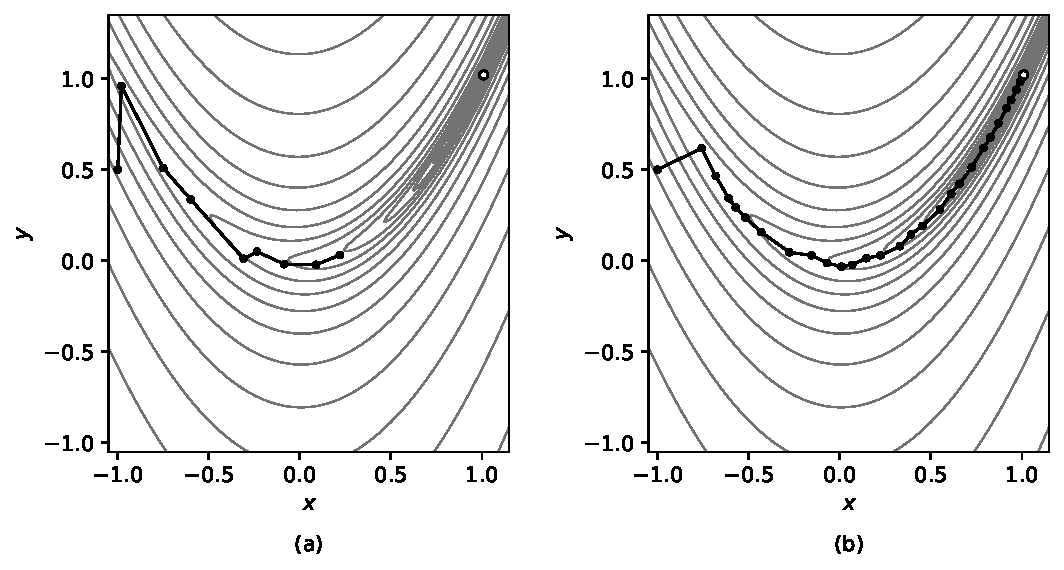
\includegraphics[width=0.94\linewidth]{figures/fig4_3_rosenbrock.pdf}
\caption{（a）Newton 法；（b）拟 Newton 法。等值线为对数标度}
\label{fig:rosenbrock-paths}
\end{figure}

\begin{exerciseBox}[练习 4.1]
试实现 DFP 方法，并利用香蕉函数测试它的收敛行为。
\end{exerciseBox}

\section{非线性方程组：零点与约束优化}

对于非线性方程组
\begin{equation}
\begin{cases}
f_1(x_1,x_2,\ldots,x_n)=0,\\
f_2(x_1,x_2,\ldots,x_n)=0,\\
\qquad\cdots\cdots\\
f_n(x_1,x_2,\ldots,x_n)=0,
\end{cases}
\tag{4.2.1}
\end{equation}
或者用向量记号写作
\begin{equation}
F(x)=0,
\tag{4.2.2}
\end{equation}
我们可以构造函数 $f(x)=F^{\mathrm T}(x)F(x)$，这样非线性方程组就转换成了 $f(x)$ 的非线性优化问题，可以用上一节介绍过的算法求解。不过，我们依旧期待寻找一些关于这类问题特别的算法。

\subsection{Newton 法}

首先，一维非线性方程的 Newton 法在此依旧适用。我们将目标函数在迭代点附近做一阶 Taylor 展开：
\begin{equation}
F(x+p)\approx F(x)+Jp,
\tag{4.2.3}
\end{equation}
其中 $(J)_{ij}=\partial_{x_j}f_i$ 为目标函数在 $x$ 处的 Jacobian 矩阵。这样，原问题便被近似成一个线性代数方程组，可以直接写出解：
\begin{equation}
p=-J^{-1}F(x).
\tag{4.2.4}
\end{equation}
与非线性优化问题中的 Newton 法类似，我们通常只将 $p$ 用作迭代方向，并在该方向上进行一维搜索得到最优步长。不过，此时一般不可能通过调节一个参数 $\alpha$ 使得方程组
\begin{equation}
F(x+\alpha p)=0
\tag{4.2.5}
\end{equation}
成立。这时，我们可以退而求其次，仅要求上式与出发点处函数正交：
\begin{equation}
F(x)^{\mathrm T}F(x+\alpha p)=0.
\tag{4.2.6}
\end{equation}

\subsection{拟 Newton 法}

与优化问题中 Newton 法的困难一样，每步迭代都计算一次 Jacobian 矩阵并不容易，从而我们需要思考如何在迭代的过程中维护一个近似的 Jacobian 矩阵，利用每一步的信息来优化和更新。记第 $k$ 步迭代中 Jacobian 矩阵的近似值为 $M_k$，我们有拟 Newton 条件
\begin{equation}
M_{k+1}s_k=y_k.
\tag{4.2.7}
\end{equation}
这里有 $s_k=x_{k+1}-x_k$，$y_k=F(x_{k+1})-F(x_k)$。注意到
\begin{equation}
(M_{k+1}-M_k)s_k=y_k-M_k s_k,
\tag{4.2.8}
\end{equation}
因此，一个自然的选择是
\begin{equation}
M_{k+1}=M_k+\frac{(y_k-M_k s_k)s_k^{\mathrm T}}{s_k^{\mathrm T}s_k}.
\tag{4.2.9}
\end{equation}
这就是非线性方程组拟 Newton 法中的 Broyden 格式。事实上，对于任意满足拟 Newton 条件 (4.2.7) 的矩阵 $M$，Broyden 格式使得矩阵修正量 $M_{k+1}-M_k$ 的 Frobenius 范数取极小。证明是直截了当的：
\begin{align}
\|M_{k+1}-M_k\|_{\mathrm F}
&=\left\|\frac{(y_k-M_k s_k)s_k^{\mathrm T}}{s_k^{\mathrm T}s_k}\right\|_{\mathrm F}\notag\\
&=\left\|\frac{(M-M_k)s_k s_k^{\mathrm T}}{s_k^{\mathrm T}s_k}\right\|_{\mathrm F}\notag\\
&\le \|M-M_k\|_{\mathrm F}\left\|\frac{s_k s_k^{\mathrm T}}{s_k^{\mathrm T}s_k}\right\|_{\mathrm F}\notag\\
&=\|M-M_k\|_{\mathrm F}.
\tag{4.2.10}
\end{align}
从而命题得证。

在计算上，我们需要的实际是 Jacobian 矩阵的逆 $W_k$。利用 Sherman--Morrison 公式
\begin{equation}
(A+xy^{\mathrm T})^{-1}=A^{-1}-\frac{A^{-1}xy^{\mathrm T}A^{-1}}{1+y^{\mathrm T}A^{-1}x},
\tag{4.2.11}
\end{equation}
可以得到 $W_k$ 的更新格式
\begin{equation}
W_{k+1}=W_k+\frac{s_k-W_k y_k}{s_k^{\mathrm T}W_k y_k}s_k^{\mathrm T}W_k.
\tag{4.2.12}
\end{equation}
同非线性优化问题中的 DFP 方法与 BFGS 方法之间的对偶一样，Broyden 方法存在着其对偶形式
\begin{equation}
W_{k+1}=W_k+\frac{(s_k-W_k y_k)y_k^{\mathrm T}}{y_k^{\mathrm T}y_k},
\tag{4.2.13}
\end{equation}
同样满足拟 Newton 条件。\jiaokan{原式 (4.2.13) 将分子印成 $y_k^{\mathrm T}(s_k-W_k y_k)$，这是标量，无法与矩阵 $W_k$ 相加；按拟 Newton 条件 $W_{k+1}y_k=s_k$ 及 Broyden 对偶更新的标准形式，应为 $(s_k-W_k y_k)y_k^{\mathrm T}$。}

\subsection{同伦方法}

从 Newton 法衍生出的各种算法的一个难点就在于，收敛不稳定。利用一个点附近的信息找到对零点的估计，移动到估计的“零点”后又发现与真实的零点相距较远。为了提高收敛的稳定性，让迭代过程中每一步移动得不是那么远，人们提出了同伦（homotopy）方法。

我们以一维求根问题 $f(x)=0$ 为例。先寻找一个简单的函数 $g(x)$，要求它容易计算、零点解析已知，且行为与 $f(x)$ 尽可能相近。然后，我们构造函数
\begin{equation}
h(x,\lambda)\equiv(1-\lambda)g(x)+\lambda f(x),\qquad \lambda\in[0,1]
\tag{4.2.14}
\end{equation}
来求解 $h(x,\lambda)$ 的零点。当 $\lambda=0$ 时，其零点就是 $g(x)$ 的零点，解析已知。随着 $\lambda$ 逐渐增加，$h(x,\lambda)$ 的零点应当也是逐渐变化的。从而我们可以构造序列 $0=\lambda_1<\lambda_2<\cdots<\lambda_n=1$，以上一步得到的零点估计 $x^*(\lambda_k)$ 作为下一步迭代的初值。由于每一步的迭代初值都相当靠近目标点，收敛应该相当快。

此外，由于 $h(x,\lambda)$ 形式简洁，导数信息也是可以复用的：
\begin{equation}
h^{(n)}(x,\lambda_k)
=\frac{\lambda_k}{\lambda_{k-1}}h^{(n)}(x,\lambda_{k-1})
-\frac{\lambda_k-\lambda_{k-1}}{\lambda_{k-1}}g^{(n)}(x).
\tag{4.2.15}
\end{equation}
同伦方法可以形象地理解成“顺藤摸瓜”：瓜（零点）在哪里儿不知道，但我可以牵出一条藤 $x^*(\lambda)$ 来，从一端 $x^*(0)$ 开始顺着往下摸，应当总能摸到瓜 $x^*(1)$ 在哪儿。这个思想可以应用到很多其他类型的数值问题上。

但不幸的是，即便对于一维求根问题，同伦方法也不能保证达到目的。函数零点在演化的过程中可能会出现一些意料之外的情况。例如考虑函数 $f(x)=x^3-x$，取 $g(x)=x$，那么当 $\lambda$ 从 0 增大到 0.5 时，一个根就会岔开变成三个根。若此时取 $g(x)=-x^3$，还能看到方程的根跑到无穷远处。这些情形示意性地绘制于图 4.4 中。

\begin{figure}[htbp]
\centering
\begin{tikzpicture}[x=5.0cm,y=1.35cm,>=Latex]
  \draw[->] (0,0) -- (1.05,0) node[right] {$\lambda$};
  \draw[->] (0,-2.1) -- (0,2.1);
  \draw[thick,domain=0:0.49,samples=80] plot (\x,{0});
  \draw[thick,domain=0.505:1,samples=100] plot (\x,{sqrt((2*\x-1)/\x)});
  \draw[thick,domain=0.505:1,samples=100] plot (\x,{-sqrt((2*\x-1)/\x)});
  \draw[thick,domain=0:0.49,samples=80] plot (\x,{0.55/sqrt(1-2*\x)});
  \draw[thick,domain=0:0.49,samples=80] plot (\x,{-0.55/sqrt(1-2*\x)});
  \draw[thin] (0,0.55) .. controls (0.35,0.72) and (0.62,0.65) .. (1,0.68);
  \draw[thin] (0,-0.55) .. controls (0.35,-0.72) and (0.62,-0.65) .. (1,-0.68);
  \node[below] at (0.5,0) {$0.5$};
\end{tikzpicture}
\caption{一些典型的同伦路径}
\label{fig:homotopy-paths}
\end{figure}

\subsection{约束优化}

在 4.1 节开头讨论的 Thomson 问题实际上是一个约束优化问题，我们通过坐标变换 $(x,y,z)\to(r,\theta,\phi)$ 将约束化到一个变量 $r=1$ 上。但对于更一般化的问题，这类变量代换并不是始终存在的。因此，我们考虑问题
\begin{equation}
\min_{x\in\mathbb R^n}f(x)\qquad\text{使得}\qquad c(x)=0,
\tag{4.2.16}
\end{equation}
其中 $c$ 为一个 $m$ 维的向量函数。这相当于我们在求解一个优化问题的同时，还要保证求得的解满足一个非线性方程组。

解析上，处理约束优化问题的标准策略是利用 Lagrange 乘子消去约束。上述问题等价于关于 $n+m$ 维向量 $z\equiv\binom{x}{\lambda}$ 的函数
\begin{equation}
L(z)=f(x)+c(x)^{\mathrm T}\lambda
\tag{4.2.17}
\end{equation}
的极值问题。不过，这样构造得到的 Lagrange 目标函数是无下界的，目标点并非其最值点，而只是驻点。从而我们无法使用前述的数值优化算法，而必须将其当作一个 $n+m$ 维非线性方程组来求解：
\begin{equation}
\begin{cases}
\nabla\!\bigl[f(x)+c(x)^{\mathrm T}\lambda\bigr]=0,\\
c(x)=0.
\end{cases}
\tag{4.2.18}
\end{equation}
记 $M\equiv\nabla\nabla[f(x)+c(x)^{\mathrm T}\lambda]$，$J\equiv\nabla c(x)$。Newton 法给出位移所满足的方程
\begin{equation}
\begin{pmatrix}M&J^{\mathrm T}\\J&0\end{pmatrix}
\begin{pmatrix}\delta x\\\delta\lambda\end{pmatrix}
=-\begin{pmatrix}\nabla f(x)+J^{\mathrm T}\lambda\\c(x)\end{pmatrix}.
\tag{4.2.19}
\end{equation}
然后反复用这组方程进行迭代即可。当然，同样可以引入线搜索和拟 Newton 法。这套方案被称为 Lagrange--Newton 法。

原则上，引入约束将问题的维度从 $n$ 降低至 $n-m$，然而 Lagrange 乘子法却反过来将维度扩张至 $n+m$。这看起来就很不划算。一种解决方案被称为罚函数（penalty function）法。我们构造函数
\begin{equation}
h(x;\sigma)=f(x)+\sigma c(x)^{\mathrm T}c(x),
\tag{4.2.20}
\end{equation}
其中附加项 $\sigma c(x)^{\mathrm T}c(x)$ 被称为罚函数。其想法在于当约束不被满足时给予一定的“惩罚”，而偏离约束越远，惩罚越大。显然，$\sigma=0$ 对应于 $f(x)$ 的无约束优化，而 $\sigma\to\infty$ 对应于需要求解的约束优化问题。那么，基于同伦方法的思想，我们应当可以从无约束优化的解一路找到待求的约束优化的解。

除去等式约束外，实际问题中还可能会抽象出不等式约束
\begin{equation}
c_i(x)>0.
\tag{4.2.21}
\end{equation}
这类问题的求解往往会更加困难。罚函数方法可以用于求解这类问题，求解方案包括内点法和外点法两类。内点法所对应的罚函数往往定义域局限在约束范围内，且越靠近约束边界，惩罚越大。一个常见的内点罚函数是
\[
p(x)=-\frac1\sigma\sum_i\ln[c_i(x)],
\]
当 $\sigma\to\infty$ 时约束范围内的惩罚归零。外点法则相反，其所构造的罚函数在约束范围内为零，而在约束范围之外，越靠近约束边界函数值越小。一个常见的外点罚函数为
\[
p(x)=\sigma\sum_i c_i^2(x)\Theta[-c_i(x)],
\]
当 $\sigma\to\infty$ 时约束范围外的惩罚趋于无穷。一般而言，如果希望找寻在约束范围内部的极值点，内点法比较合适，而如果希望找寻在边界附近的极值点，外点法则更好用。

如果待优化函数为线性函数，且不等式约束均为线性的约束，则相应的数值问题退化为线性规划问题。目前处理这类问题通行的方法是单纯形法，有需要的读者可以阅读参考书 [6] 的第三章。

\begin{exerciseBox}[练习 4.2]
设有一简谐振子 $A$，其运动由下式给出：
\[
x(t)=x_0\cos\omega t.
\]
振子上束缚有一质点 $E$，其质量 $m_E$ 远小于该振子。在 $t=t_i$ 时刻解除束缚，该质点以速度 $-\omega x_0\sin\omega t_i$ 做匀速直线运动。当 $t=t_r$ 时，$A$ 与 $E$ 再次相遇：
\[
x_0\cos\omega t_r=x_0\cos\omega t_i-\omega(t_r-t_i)x_0\sin\omega t_i.
\]
进而发生碰撞。试利用本节所给出的算法求解如下两个约束极值问题：
\begin{enumerate}[label=(\arabic*)]
\item $t_i$ 与 $t_r$ 取多大时，碰撞发生时质点相对振子的动能最大？最大为多少？
\item 设碰撞是完全弹性的，那么 $t_i$ 与 $t_r$ 取多大时，碰撞结束后质点的动能最大？最大为多少？
\end{enumerate}
这个问题与强激光场下原子的电离动力学密切相关。
\end{exerciseBox}

\section{常微分方程组：Runge--Kutta 算法}

在 3.4 节中，我们以电路网络作为引子，探讨了线性常微分方程组
\begin{equation}
\dot x(t)=Ax(t)
\tag{4.3.1}
\end{equation}
的求解。在这种情况下，我们只需要进行一次矩阵对角化，就能得到方程在任意 $t$ 时刻的解。然而，即使是电路，其中依旧可能包含着一些诸如二极管之类的非线性器件。

例如图 4.5 所示的蔡氏电路，$N_R$ 是一个有着非线性负阻特性的蔡氏二极管。其目的是在电路中模拟混沌现象。此时，我们面临的是非线性常微分方程组
\begin{equation}
\begin{cases}
\dot y(t)=f[t,y(t)],\\
y(t_0)=y_0.
\end{cases}
\tag{4.3.2}
\end{equation}
当然，在 2.6 节中，我们已经接触了一些简单的算法。但那些算法都不存在可拓展性，想提高精度只能不断降低步长。这种做法在面临一些困难的问题时会变得低效。本节中我们将介绍一些更高阶的算法，它们通常在每一步上需要更多的计算消耗，但可以容许更大的步长，从而整体上在保证精度的同时减少了计算量。\footnote{与上一节中的算法同名，但它们是完全不同的算法。}



\begin{figure}[htbp]
\centering
\begin{tikzpicture}[x=1.05cm,y=1.0cm,>=Latex]
  % bottom bus
  \draw[thick] (0,0)--(6.2,0);
  % top buses and series resistor
  \draw[thick] (0,2.2)--(2.5,2.2);
  \draw[thick] (3.7,2.2)--(6.2,2.2);
  \draw[thick] (2.5,2.2)--(2.75,2.2);
  \draw[thick] (3.45,2.2)--(3.7,2.2);
  \draw[thick,decorate,decoration={zigzag,segment length=3.5pt,amplitude=2pt}] (2.75,2.2)--(3.45,2.2);
  \node[above] at (3.1,2.2) {$R$};
  % inductor L
  \draw[thick] (0.45,2.2)--(0.45,1.95);
  \draw[thick,decorate,decoration={coil,segment length=4pt,amplitude=4pt,aspect=0.55}] (0.45,1.95)--(0.45,0.25);
  \draw[thick] (0.45,0.25)--(0.45,0);
  \node[left] at (0.25,1.1) {$L$};
  % C2
  \draw[thick] (1.75,2.2)--(1.75,1.35);
  \draw[thick] (1.48,1.35)--(2.02,1.35);
  \draw[thick] (1.48,1.12)--(2.02,1.12);
  \draw[thick] (1.75,1.12)--(1.75,0);
  \node[right] at (1.95,1.7) {$C_2$};
  % C1
  \draw[thick] (4.45,2.2)--(4.45,1.35);
  \draw[thick] (4.18,1.35)--(4.72,1.35);
  \draw[thick] (4.18,1.12)--(4.72,1.12);
  \draw[thick] (4.45,1.12)--(4.45,0);
  \node[right] at (4.65,1.7) {$C_1$};
  % nonlinear resistor N_R
  \draw[thick] (5.65,2.2)--(5.65,1.75);
  \draw[thick] (5.35,1.75) rectangle (5.95,0.55);
  \draw[thick] (5.65,0.55)--(5.65,0);
  \node[right] at (5.95,1.15) {$N_R$};
  % nodes
  \fill (1.75,2.2) circle (1.6pt);
  \fill (4.45,2.2) circle (1.6pt);
\end{tikzpicture}
\caption{蔡氏电路}
\label{fig:chua-circuit}
\end{figure}

在正式开始之前，我们需要指出 $f[t,y(t)]$ 中对时间 $t$ 的依赖总是可以被“消掉”：我们可以引入新的函数 $y^*$，满足方程
\begin{equation}
\begin{cases}
y^{*\prime}(t)=1,\\
y^*(t_0)=t_0.
\end{cases}
\tag{4.3.3}
\end{equation}
显然，我们知道 $y^*=t$。此时将它看成 $y$ 的一个新分量，那么 $f[t,y(t)]$ 就可以完全写成关于 $y$ 的函数。因此在本节中，我们总是基于不含时的形式展开讨论。

\subsection{显式 Runge--Kutta 算法}

对于 $n$ 维一阶非线性常微分方程组，我们引入一类一般的算法：Runge--Kutta（R--K）算法
\begin{equation}
 g_i=y_{k-1}+\tau\sum_{j=1}^{m}a_{ij}f(g_j),
\tag{4.3.4}
\end{equation}
\begin{equation}
 y_k=y_{k-1}+\tau\sum_{i=1}^{m}b_i f(g_i),
\tag{4.3.5}
\end{equation}
其中 $\tau=t_k-t_{k-1}$，$a_{ij},b_i$ 为事先确定的常系数，而 $g_i$ 需要通过求解 (4.3.4) 式这个非线性自洽方程组来得到。

为了理解这个式子的含义，我们可以尝试写下方程的形式解
\begin{align}
 y_k
 &=y_{k-1}+\int_{t_{k-1}}^{t_k}f[y(t)]\,\mathrm dt\notag\\
 &\approx y_{k-1}+\tau\sum_{i=1}^{m}b_i f[y(t_{k-1}+c_i\tau)].
\tag{4.3.6}
\end{align}
观察上式可知，R--K 算法相当于在两个时间格点之间取了 $m$ 个分点 $t_{k-1}+c_i\tau$，给出这些分点上的函数 $y$ 的估计值 $g_i$，再将这样计算得到的导数按一定权重 $b_i$ 求和进行数值积分，来得到最终的函数值 $y_k$。其中需要的 $g_i$ 可以通过与 (4.3.6) 式类似的格式给出，只要将积分区间变成 $(t_{k-1},t_{k-1}+c_i\tau)$ 即可。参数 $a_{ij},b_i$ 和 $c_i$ 的选取则决定了积分估计的精度，它们至少得在 $f$ 为常函数时给出正确的结果，即
\begin{equation}
\begin{cases}
\displaystyle\sum_{j=1}^{m}a_{ij}=c_i,\\[4pt]
\displaystyle\sum_{i=1}^{m}b_i=1.
\end{cases}
\tag{4.3.7}
\end{equation}
若对任意 $j\ge i$ 有 $a_{ij}=0$，则 (4.3.4) 式可以直接逐项求解，R--K 算法成为显式算法，否则 R--K 算法为隐式算法。

为方便起见，高阶 Runge--Kutta 算法的系数常用如下形式的表格表示，称为 Butcher 表：
\begin{equation}
\begin{array}{c|cccc}
 c_1&a_{11}&a_{12}&\cdots&a_{1m}\\
 c_2&a_{21}&a_{22}&\cdots&a_{2m}\\
 \vdots&\vdots&\vdots&\ddots&\vdots\\
 c_m&a_{m1}&a_{m2}&\cdots&a_{mm}\\ \hline
 &b_1&b_2&\cdots&b_m
\end{array}
\tag{4.3.8}
\end{equation}
或简记为
\begin{equation}
\begin{array}{c|c}
 c&A\\ \hline
 &b^{\mathrm T}
\end{array}.
\tag{4.3.9}
\end{equation}
显式算法意味着 $A$ 一定是一个严格下三角矩阵，同时从 (4.3.7) 式中也可以推出 $c_1=0$。

接下来讨论如何确定 Butcher 表。我们可以通过将 $y(t_k)$ 用 $y(t_{k-1})$ 及其各阶导数的 Taylor 级数展开，与 $y_k$ 逐阶比较，通过调整系数来使得算法达到最高的截断精度。我们将以 $m=2$ 为例演示这一过程。下述诸函数若未写明自变量取值，均默认在 $t_{k-1}$ 处取值。

二阶显式 Runge--Kutta 算法写作
\begin{align}
 y_k&=y_{k-1}+\tau(b_1k_1+b_2k_2),\tag{4.3.10}\\
 k_1&=f(y_{k-1}),\tag{4.3.11}\\
 k_2&=f(y_{k-1}+\tau a_{21}k_1).\tag{4.3.12}
\end{align}
而准确的结果为
\begin{equation}
 y(t_k)=y+y'\tau+y''\frac{\tau^2}{2}+y'''\frac{\tau^3}{6}+O(\tau^4).
\tag{4.3.13}
\end{equation}
将导数逐阶写开：
\begin{equation}
\begin{cases}
 y'=f,\\
 \displaystyle y''=\frac{\mathrm df}{\mathrm dt}=f\cdot\nabla f,\\
 y'''=f\cdot\nabla f\cdot\nabla f+(f\cdot\nabla)^2f.
\end{cases}
\tag{4.3.14}
\end{equation}
另一方面，使用二阶显式 R--K 算法得到的 $y_k$ 为
\begin{align}
 y_k
 &=y+\tau\bigl[b_1f+b_2f(y+\tau a_{21}f)\bigr]\notag\\
 &=y+\tau(b_1+b_2)f+\tau^2b_2a_{21}f\cdot\nabla f
 +\frac{\tau^3}{2}b_2a_{21}^2(f\cdot\nabla)^2f+O(\tau^4).
\tag{4.3.15}
\end{align}
同样可以按照 $\tau$ 的幂次逐阶展开。相比较可以发现，若须使两式前两阶相等，使三个系数满足两个等式即可，但第三阶无论怎样也无法相等，即二阶 Runge--Kutta 算法精度最高为二阶。实践中常取 $b_1=b_2=1/2$：
\begin{equation}
\begin{array}{c|cc}
0&0&0\\
1&1&0\\ \hline
&1/2&1/2
\end{array}.
\tag{4.3.16}
\end{equation}
可以证明，当 $m\le 4$ 时算法的阶数和其最高精度相等。而当 $m$ 继续增长时，最高可能精度的增长速度会减慢。因此四阶 Runge--Kutta 算法是最常用的，下述的 R--K4 格式尤其著名：
\begin{equation}
\begin{array}{c|cccc}
0&0&0&0&0\\
1/2&1/2&0&0&0\\
1/2&0&1/2&0&0\\
1&0&0&1&0\\ \hline
&1/6&2/6&2/6&1/6
\end{array}.
\tag{4.3.17}
\end{equation}
这里的积分权值 $b_i$ 和积分格点 $c_i$ 与我们在 2.2 节中得到的 Simpson 求积公式一致。

\subsection{隐式 Runge--Kutta 算法}

如果我们不限定算法是显式的，R--K 算法很容易实现更高阶的精度。为了确定在高阶 R--K 算法中这些系数所需要满足的条件，我们考虑简化情形 $f(y)=y$，此时可以写下严格解
\begin{equation}
 \tilde g_i=e^{c_i\tau}y_{k-1}=\sum_{l=0}^{\infty}\frac{(\tau c_i)^l}{l!}y_{k-1},\qquad
 \tilde y_k=e^\tau y_{k-1}=\sum_{l=0}^{\infty}\frac{\tau^l}{l!}y_{k-1}.
\tag{4.3.18}
\end{equation}
将这两个展开式代入 R--K 算法的迭代格式 (4.3.4) 和 (4.3.5)，令 $\tau$ 的每一个幂次前的系数相等，我们可以得到
\begin{align}
 \sum_{i=1}^{m}b_i c_i^{l-1}&=\frac1l,\tag{4.3.19}\\
 \sum_{j=1}^{m}a_{ij}c_j^{l-1}&=\frac1l c_i^l.\tag{4.3.20}
\end{align}
我们记 (4.3.19) 式对于 $l\le\xi$ 成立为 $B(\xi)$，(4.3.20) 式对于 $l\le\xi$ 成立为 $C(\xi)$。同时，考虑等式
\begin{equation}
 \sum_i b_i c_i^{l-1}a_{ij}=\frac1l b_j(1-c_j^l).
\tag{4.3.21}
\end{equation}
记上式对于 $l\le\xi$ 成立为 $D(\xi)$。容易检验，$B(k+m),C(m)$ 可以导出 $D(k)$。

可以证明，如果系数 $A,b$ 满足 $B(p),C(\eta),D(\xi)$，且 $p\le\xi+\eta+1$，$p\le2\eta+2$，那么这样的 R--K 算法具有 $p$ 阶精度。\footnote{Butcher J. C. Implicit Runge--Kutta processes. \textit{Math. Comp.}, 1964, 18: 50.}

观察 (4.3.19) 式可知，如果将 $c_j$ 视作 $(0,1)$ 上的积分节点，$b_j$ 视作积分权值，那么该式就相当于要求数值积分能够精确给出 $\int_0^1x^{l-1}\,\mathrm dx$，这是容易做到的。进而对于 (4.3.20) 式中的每个 $i$，取 $l$ 从 1 到 $m$，得到 $m$ 个 $m$ 维的线性方程组，求解它们就能求得 $a_{ij}$ 的值，使其满足 $C(m)$。

从这个视角出发，我们可以按照前面讨论过的 Gauß 积分节点来选取 $c_j$。$m$ 阶 Gauß 积分具有 $2m-1$ 阶代数精度，故 $B(2m)$ 成立。再加上 $C(m)$ 和之前的结论，可以导出 $D(m)$ 成立。这样，$m$ 阶 Gauß 节点所相应的 R--K 算法具有 $2m$ 阶精度。当然，我们也可以固定一个边界点，使用 Radau 积分格点。

一阶 Gauß R--K 算法为
\begin{equation}
\text{Gauß 2:}\qquad
\begin{array}{c|c}
1/2&1/2\\ \hline
&1
\end{array},
\tag{4.3.22}
\end{equation}
与中点 Euler 法等价。

比较常用的高阶方案有如下两个：
\begin{equation}
\text{Radau 5:}\quad
\begin{array}{c|ccc}
\frac{4-\sqrt6}{10}&\frac{88-7\sqrt6}{360}&\frac{296-169\sqrt6}{1800}&\frac{-2+3\sqrt6}{225}\\[4pt]
\frac{4+\sqrt6}{10}&\frac{296+169\sqrt6}{1800}&\frac{88+7\sqrt6}{360}&\frac{-2-3\sqrt6}{225}\\[4pt]
1&\frac{16-\sqrt6}{36}&\frac{16+\sqrt6}{36}&\frac19\\ \hline
&\frac{16-\sqrt6}{36}&\frac{16+\sqrt6}{36}&\frac19
\end{array},
\tag{4.3.23}
\end{equation}
\begin{equation}
\text{Gauß 6:}\quad
\begin{array}{c|ccc}
\frac12-\frac{\sqrt{15}}{10}&\frac5{36}&\frac29-\frac{\sqrt{15}}{15}&\frac5{36}-\frac{\sqrt{15}}{30}\\[4pt]
\frac12&\frac5{36}+\frac{\sqrt{15}}{24}&\frac29&\frac5{36}-\frac{\sqrt{15}}{24}\\[4pt]
\frac12+\frac{\sqrt{15}}{10}&\frac5{36}+\frac{\sqrt{15}}{30}&\frac29+\frac{\sqrt{15}}{15}&\frac5{36}\\ \hline
&\frac5{18}&\frac49&\frac5{18}
\end{array}.
\tag{4.3.24}
\end{equation}
分别具有 5 阶和 6 阶精度。

\subsection{隐式迭代求根}

隐式算法的每一步迭代都需要求解一个 $m\times n$ 维的非线性方程组 (4.3.4) 式。不过幸运的是，由于迭代步长通常不大，方程的解 $g_i$ 一般都和 $y_{k-1}$ 相距不远，从而可以把 $y_{k-1}$ 作为 $g_i$ 的初值，通过迭代算法快速求解。

我们定义 $m\times n$ 维的双下标向量
\begin{equation}
 (G)_{i\alpha}=(g_i)_\alpha,
\tag{4.3.25}
\end{equation}
自洽方程写作
\begin{equation}
 G_{i\alpha}-(y_{k-1})_\alpha-\tau\sum_{l=1}^{m}a_{il}f_\alpha(g_l)=0.
\tag{4.3.26}
\end{equation}
将上式对 $G_{j\beta}$ 求偏导数，可以得到整个非线性方程组的 Jacobian 矩阵
\begin{equation}
 (K)_{j\beta,i\alpha}=\delta_{ij}\delta_{\alpha\beta}-\tau a_{ij}(J_i)_{\beta\alpha},
\tag{4.3.27}
\end{equation}
其中 $J_i$ 是 $f(y)$ 在 $y=g_i$ 处的 Jacobian 矩阵。作为一个估计，我们令各处的 Jacobian 矩阵近似相等，
\begin{equation}
 (J_i)_{\beta\alpha}\approx\left.\frac{\partial f_\alpha(y)}{\partial y_\beta}\right|_{y=y_{k-1}}.
\tag{4.3.28}
\end{equation}
这样 $K$ 便成了一个常量，从而 Newton 迭代格式为
\begin{equation}
 \Delta G_{i\alpha}
 =\sum_{j=1}^{m}\sum_{\beta=1}^{n}(K^{-1})_{i\alpha,j\beta}
 \left[G_{j\beta}-(y_{k-1})_\beta-\tau\sum_{l=1}^{m}a_{jl}f_\beta(g_l)\right].
\tag{4.3.29}
\end{equation}
单次计算便能得到在近似意义下所需要的解。另一种改进的策略是，将前述 $K$ 作为 Jacobian 矩阵的初始猜测，然后使用拟 Newton 法来不断更新改善。

\subsection{稳定性分析}

我们来讨论一下 R--K 算法的稳定性。作为一个例子，将 R--K 算法应用于方程 $y'=\lambda y$ 上，并取 $y(t_n)=y_n+\varepsilon_n$，有
\begin{equation}
\begin{cases}
\displaystyle \delta_i=\varepsilon_{n-1}+\lambda\tau\sum_{j=1}^{m}a_{ij}\delta_j,\\[5pt]
\displaystyle \varepsilon_n=\varepsilon_{n-1}+\lambda\tau\sum_{i=1}^{m}b_i\delta_i,
\end{cases}
\tag{4.3.30}
\end{equation}
其中 $\delta_i$ 是计算 $f(g_i)$ 时的误差。计算误差的模方
\begin{align}
 |\varepsilon_n|^2
 &=|\varepsilon_{n-1}|^2+2\Re(\lambda\tau)\sum_i b_i\delta_i\delta_{n-1}^*
   +|\lambda\tau|^2\sum_{i,j}b_ib_j\delta_i\delta_j^*\notag\\
 &=|\varepsilon_{n-1}|^2+2\Re(\lambda\tau)\sum_i b_i|\delta_i|^2\notag\\
 &\quad+|\lambda\tau|^2\sum_{i,j}(b_ib_j-b_i a_{ij}-b_j a_{ji})\delta_i\delta_j^*.
\tag{4.3.31}
\end{align}
注意到 $b_i$ 相当于积分权值，通常大于零。如果有 $\Re\lambda<0$，再加上矩阵
\[
 (M)_{ij}=b_j a_{ji}+b_i a_{ij}-b_i b_j
\]
半正定，我们就得到
\begin{equation}
 |\varepsilon_n|^2\le |\varepsilon_{n-1}|^2.
\tag{4.3.32}
\end{equation}
误差不会随着迭代而增长，从而算法是稳定的。那么回忆之前的定义，若矩阵 $M$ 半正定，则 R--K 算法的稳定域包含左半平面，这类 R--K 算法是 A--稳定的。可以证明，不存在 A--稳定的显式 R--K 算法。

给矩阵 $M$ 右乘 $c_j^{l-1}$，有
\begin{equation}
 \sum_{j=1}^{m}(b_i b_j-b_i a_{ij}-a_{ji}b_j)c_j^{l-1}
 =b_i\frac1l-b_i\frac{c_i^l}{l}-\frac1l b_i(1-c_i^l)=0.
\tag{4.3.33}
\end{equation}
推导中用到了 $B(l),C(l)$ 和 $D(l)$。如果上式对于 $l=1,\ldots,m$ 均成立，则 $M$ 是零矩阵。从而，基于 Gauß 积分格点的隐式 R--K 算法都是 A--稳定的。

\subsection{数值实验}

我们以 Kepler 问题为例测试 R--K4 算法：
\begin{equation}
\begin{cases}
 x'=p_x,\\
 y'=p_y,\\
 p_x'=-x/(x^2+y^2)^{3/2},\\
 p_y'=-y/(x^2+y^2)^{3/2},
\end{cases}
\tag{4.3.34}
\end{equation}
初始条件取作
\[
 x|_{t=0}=1,
 \qquad y|_{t=0}=0,
 \qquad p_x|_{t=0}=0,
 \qquad p_y|_{t=0}=1.3.
\]
对于这类问题，检验算法精度最有效的方法便是计算那些解析给出的守恒量在数值求解过程中是否依旧守恒。在 Kepler 问题中，我们有三个独立守恒量：能量
\begin{equation}
 E=\frac{p_x^2+p_y^2}{2}-\frac1{\sqrt{x^2+y^2}},
\tag{4.3.35}
\end{equation}
角动量的 $z$ 分量
\begin{equation}
 J_z=xp_y-yp_x,
\tag{4.3.36}
\end{equation}
以及 Laplace--Runge--Lenz 矢量的 $x$ 分量
\begin{equation}
 L_x=p_yJ_z-\frac{x}{\sqrt{x^2+y^2}}.
\tag{4.3.37}
\end{equation}
我们分别采用中点 Euler 法和 R--K4 来求解这个问题，并将相应求得的守恒量随时间的变化绘制于图 4.6 中。从能量的变化中可以看到，具有四阶精度的 R--K4 显然远优于仅有二阶精度的中点 Euler 法，并且这个差异在步长减半之后更加明显了。不过，中点 Euler 法给出的能量虽然抖动较大，却在演化过程中始终做周期变化，而更高精度的 R--K4 反而在单向漂移。对于角动量，事情更是反过来了，中点 Euler 法给出了数值精度内完全不变的角动量，而 R--K4 依旧呈现出单调的漂移行为。只有在 Laplace--Runge--Lenz 矢量上，R--K4 才表现出了无可争议的优势。

这些看似奇怪的数值行为，其背后实际上都有着清晰的理论解释。掌握这些规律，借此设计更高效的算法以便于求解实际物理问题，这便是我们下一节将要探讨的内容：辛算法。

\begin{figure}[htbp]
\centering
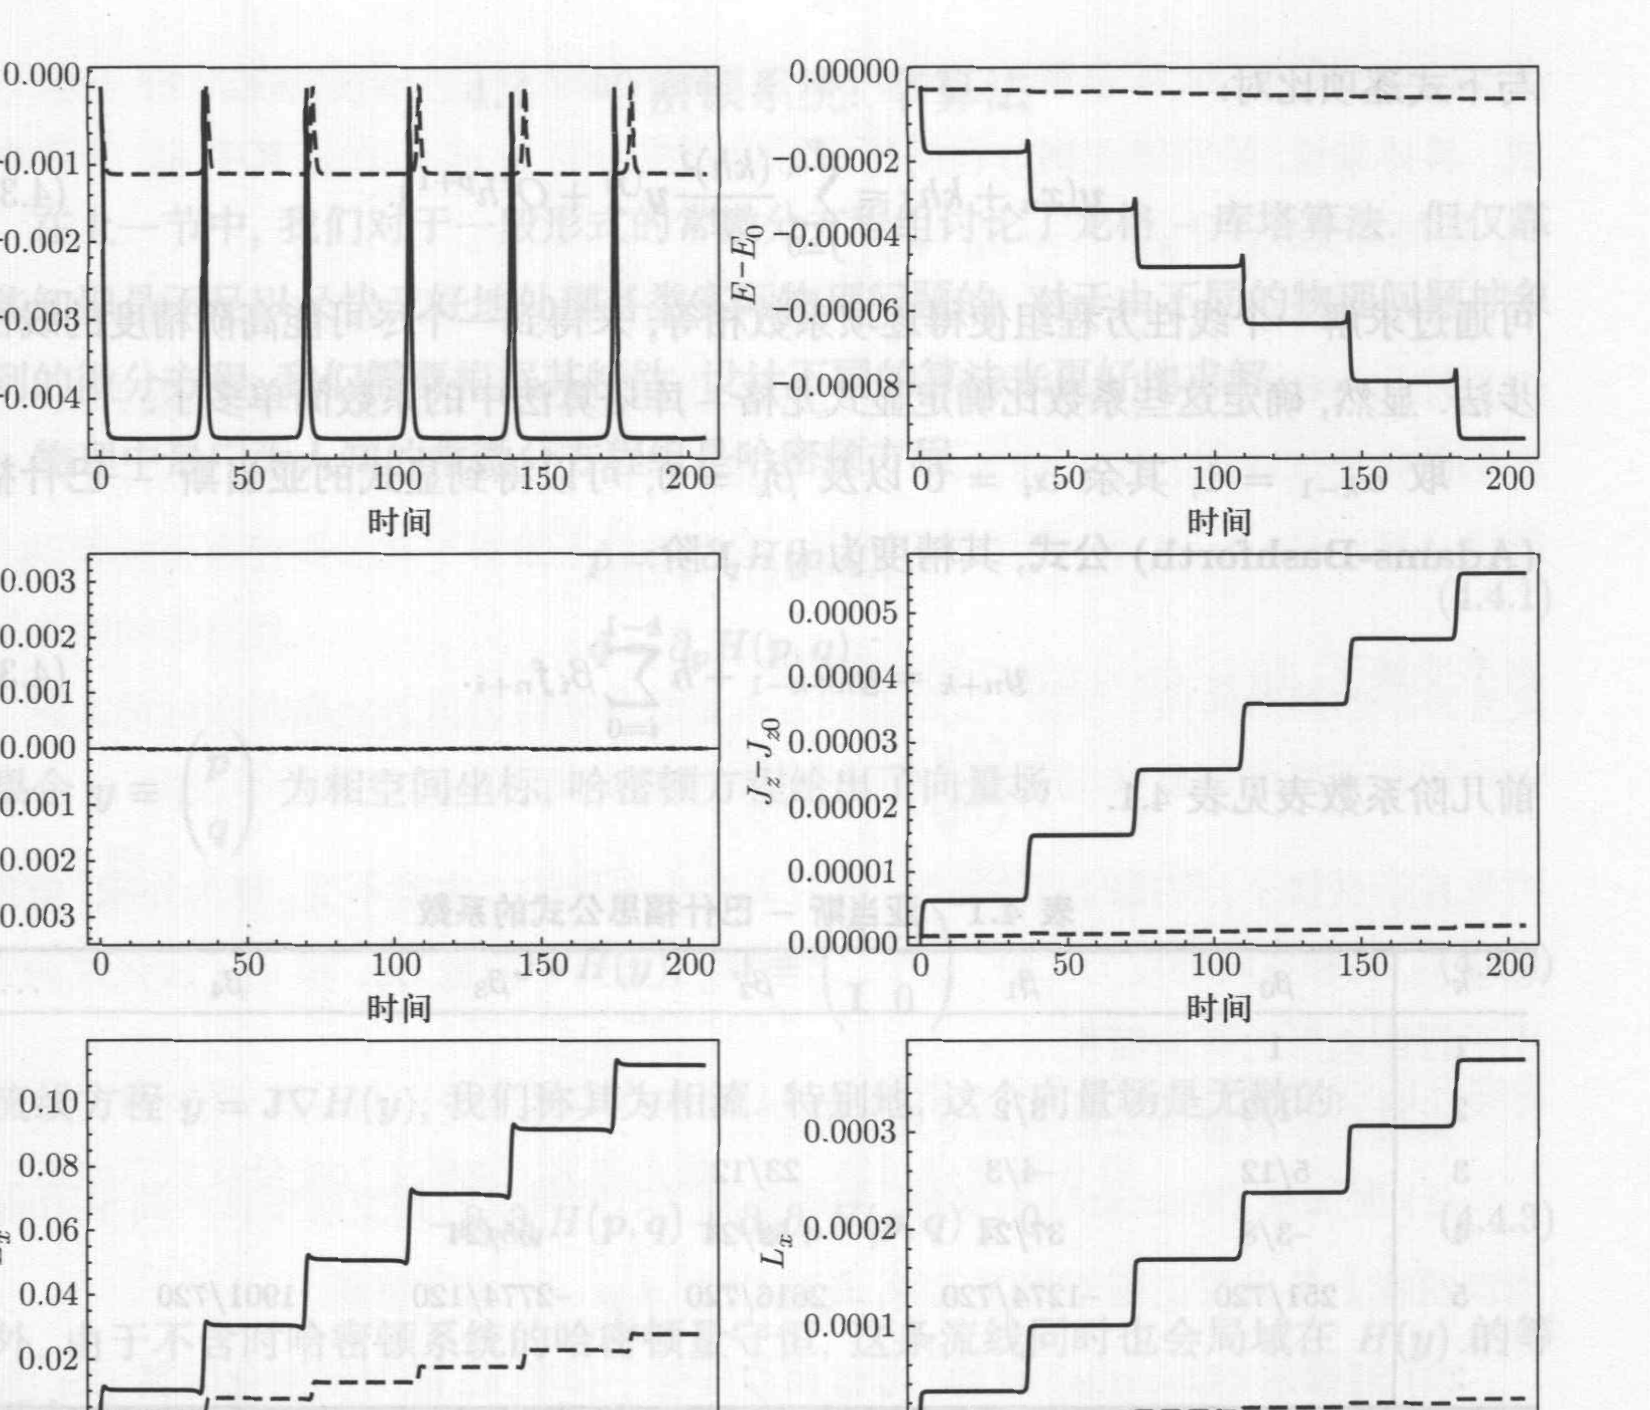
\includegraphics[width=0.88\linewidth]{figures/fig4_6_kepler.png}
\caption{Runge--Kutta 算法求解 Kepler 问题。左列为中点 Euler 法的结果，右列为 R--K4 的结果。从上至下三行分别为能量、角动量与 Laplace--Runge--Lenz 矢量与零时刻的差值。虚线和实线分别代表时间步长取 0.1 和 0.2 的情形}
\label{fig:rk-kepler}
\end{figure}

\subsection{线性多步法}

在 R--K 算法中，虽然涉及了函数在节点 $t+c_i\tau$ 上的估计值 $g_i$，但 $g_i$ 依旧是由 $y_{k-1}$ 得到的。像这种在计算下一步 $y_k$ 时只用到了上一步 $y_{k-1}$ 信息的算法被称为单步法。那么与之对应的还有多步法。当然，由于多步法涉及之前若干个格点的信息，它是无法自启动的，通常需要通过单步法来计算前几步。另外，由于对之前格点信息的利用涉及其与此处的距离，因此变步长技术很难应用到多步法之中，而常用固定步长 $h$。

一般的线性多步法公式表示为
\begin{equation}
 y_{n+k}=\sum_{i=0}^{k-1}\alpha_i y_{n+i}+h\sum_{i=0}^{k}\beta_i f_{n+i}.
\tag{4.3.38}
\end{equation}
根据 $\beta_k$ 是否为零，多步法分为显式多步法和隐式多步法。从上式出发进行逐阶展开
\begin{align}
 y_{n+k}
 &=\sum_{i=0}^{k-1}\alpha_i y(t_n+ih)+h\sum_{i=0}^{k}\beta_i y'(t_n+ih)\notag\\
 &=\sum_{j=0}^{p}\frac{h^j}{j!}y^{(j)}
 \left[\sum_{i=0}^{k-1}\bigl(\alpha_i i^j+j\beta_i i^{j-1}\bigr)+j\beta_k k^{j-1}\right]+O(h^{p+1}),
\tag{4.3.39}
\end{align}
与下式逐项比较：
\begin{equation}
 y(x_n+kh)=\sum_{j=0}^{p}\frac{(kh)^j}{j!}y^{(j)}+O(h^{p+1}).
\tag{4.3.40}
\end{equation}
可通过求解一个线性方程组使得逐项系数相等，来得到一个尽可能高阶精度的线性多步法。显然，确定这些系数比确定显式 Runge--Kutta 算法中的系数简单多了。

取 $\alpha_{k-1}=1$，其余 $\alpha_i=0$ 以及 $\beta_k=0$，可以得到显式的 Adams--Bashforth 公式，其精度为 $k-1$ 阶：
\begin{equation}
 y_{n+k}=y_{n+k-1}+h\sum_{i=0}^{k-1}\beta_i f_{n+i}.
\tag{4.3.41}
\end{equation}
前几阶系数表见表 4.1。

\begin{table}[htbp]
\centering
\caption{Adams--Bashforth 公式的系数}
\begin{tabular}{c c c c c c c}
\toprule
$k$&$\beta_0$&$\beta_1$&$\beta_2$&$\beta_3$&$\beta_4$&$\cdots$\\
\midrule
1&$1$&&&&&\\
2&$-1/2$&$3/2$&&&&\\
3&$5/12$&$-4/3$&$23/12$&&&\\
4&$-3/8$&$37/24$&$-59/24$&$55/24$&&\\
5&$251/720$&$-1274/720$&$2616/720$&$-2774/720$\footnotemark&$1901/720$&\\
$\vdots$&&&$\vdots$&&&\\
\bottomrule
\end{tabular}
\end{table}
\footnotetext{\textbf{校勘：}表 4.1 的 $k=5$ 行中，原印本将 $\beta_3$ 印为 $-2774/120$。由五阶 Adams--Bashforth 公式的标准系数，且与同一行其余统一以 720 为分母的写法一致，此处应为 $-2774/720=-1387/360$。}

取 $\alpha_{k-1}=1$，其余 $\alpha_i=0$，可以得到隐式的 Adams--Moulton 公式，其精度为 $k$ 阶：
\begin{equation}
 y_{n+k}=y_{n+k-1}+h\sum_{i=0}^{k}\beta_i f_{n+i}.
\tag{4.3.42}
\end{equation}
前几阶系数表见表 4.2。

\begin{table}[htbp]
\centering
\caption{Adams--Moulton 公式的系数}
\begin{tabular}{c c c c c c c c}
\toprule
$k$&$\beta_0$&$\beta_1$&$\beta_2$&$\beta_3$&$\beta_4$&$\beta_5$&$\cdots$\\
\midrule
1&$1/2$&$1/2$&&&&&\\
2&$-1/12$&$2/3$&$5/12$&&&&\\
3&$1/24$&$-5/24$&$19/24$&$3/8$&&&\\
4&$-19/720$&$53/360$&$-11/30$&$323/360$&$251/720$&&\\
5&$3/160$&$-173/1440$&$241/720$&$-133/240$&$1427/1440$&$95/288$&\\
$\vdots$&&&&$\vdots$&&&\\
\bottomrule
\end{tabular}
\end{table}

当 $f$ 不依赖于 $y$ 时，Adams 类公式等价于 Newton--Cotes 积分法。

\section{Hamilton 系统：辛算法}

在上一节中，我们对于一般形式的常微分方程组讨论了 Runge--Kutta 算法。但仅靠这些知识是不足以又快又好地处理各类实际物理问题的。对于由不同的物理问题抽象得到的微分方程，我们需要根据其特性，设计不同的算法来更好地求解。

物理中最广为人知的常微分方程组是 Hamilton 方程
\begin{equation}
\dot p=-\partial_qH(p,q),\qquad
\dot q=\partial_pH(p,q).
\tag{4.4.1}
\end{equation}
如果令 $y\equiv\binom pq$ 为相空间坐标，Hamilton 方程给出了向量场
\begin{equation}
J\nabla H(y),\qquad
J=\begin{pmatrix}0&-I\\I&0\end{pmatrix},
\tag{4.4.2}
\end{equation}
的流线方程 $\dot y=J\nabla H(y)$，我们称其为相流。特别地，这个向量场是无散的：
\begin{equation}
-\partial_p\partial_qH(p,q)+\partial_q\partial_pH(p,q)=0.
\tag{4.4.3}
\end{equation}
此外，由于不含时 Hamilton 系统的 Hamilton 量守恒，这条流线同时也会局域在 $H(y)$ 的等值面上。

本节中，我们将先简略地回顾一下理论力学的知识，介绍 Hamilton 方程解的特殊结构，然后讨论如何设计算法，使得这些特殊结构能够得到保留。

\subsection{Hamilton 正则方程的辛结构}

考虑变换 $S:y\to\tilde y$。在这个变换下，Hamilton 方程变为
\begin{equation}
\frac{\partial y}{\partial\tilde y}\frac{\partial\tilde y}{\partial t}
=J\left(\frac{\partial\tilde y}{\partial y}\right)^{\!\mathrm T}\frac{\partial H}{\partial\tilde y},
\qquad
\frac{\partial\tilde y}{\partial t}
=\frac{\partial\tilde y}{\partial y}J\left(\frac{\partial\tilde y}{\partial y}\right)^{\!\mathrm T}\frac{\partial H}{\partial\tilde y}.
\tag{4.4.4}
\end{equation}
如果有等式
\begin{equation}
\frac{\partial\tilde y}{\partial y}J\left(\frac{\partial\tilde y}{\partial y}\right)^{\!\mathrm T}=J
\tag{4.4.5}
\end{equation}
恒成立，那么 Hamilton 方程形式不变。这样的变换 $S$ 被称为辛变换，相应的 Jacobian 矩阵 $\partial y/\partial\tilde y$ 称为辛矩阵。显然，时间平移变换 $S:y(t)\to\tilde y(t)=y(t+\Delta t)$ 就是一个辛变换。

通过规定辛变换之间的乘积为复合，可以检验 $\mathbb R^{2n}$ 上的全体辛变换构成一个李群，记作 $\operatorname{Sp}(2n)$，称为 $2n$ 阶辛群。这样，Hamilton 正则方程的解由一个单参数辛群 $\{g_H^t;t\}$ 生成。具体来说，Hamilton 正则方程的传播可以写成 $y(t)=g_H^t(y(0))$，其中 $g_H^t$ 为辛变换：$g_H^0$ 是恒等变换，而 $g_H^{t_1+t_2}=g_H^{t_1}\cdot g_H^{t_2}$。

Hamilton 方程在辛变换下不变，对应着一个对称性，而对称性意味着守恒量，这个守恒量被称为辛结构。以相空间中一点 $y$ 为起始点引出两个无穷小向量 $\mathrm dy_1,\mathrm dy_2$，考虑它们的一个二次型
\begin{equation}
\omega\equiv(\mathrm dy_1)^{\mathrm T}J\,\mathrm dy_2.
\tag{4.4.6}
\end{equation}
在辛变换下，$\mathrm d\tilde y\leftarrow \mathrm dy=(\partial y/\partial\tilde y)\mathrm d\tilde y$，那么
\begin{equation}
\omega=\mathrm d\tilde y_1^{\mathrm T}
\left(\frac{\partial y}{\partial\tilde y}\right)^{\!\mathrm T}
J\left(\frac{\partial y}{\partial\tilde y}\right)\mathrm d\tilde y_2
=\mathrm d\tilde y_1^{\mathrm T}J\,\mathrm d\tilde y_2\equiv\tilde\omega.
\tag{4.4.7}
\end{equation}
可见在辛变换下，即随时间传播时，这对无穷小向量的二次型不变，称为外积。值得注意的是，在相空间维度为二时，这个二次型等于无穷小向量 $\mathrm dy_1$ 和 $\mathrm dy_2$ 所张成的无穷小平行四边形的有向面积。

由这个守恒量可以证明如下几个推论：
\begin{enumerate}[label=(\arabic*)]
\item Poincaré 不变量：考虑扩展了时间维度的相空间中任一简单闭曲线，当该曲线上各点按正则方程演化时，环路积分 $\oint p\cdot\mathrm dq$ 为守恒量。
\item Liouville 定理：考虑相空间任一体积元，随时间演化时其（$2n$ 维的）体积不变。
\end{enumerate}

当 Hamilton 量是广义动量和广义坐标的二次型时，微分形式的辛结构守恒可以拓展到相空间坐标自身，即
\begin{equation}
 y_1^{\mathrm T}Jy_2=q_1^{\mathrm T}p_2-p_1^{\mathrm T}q_2
\tag{4.4.8}
\end{equation}
守恒。这个量形式上与角动量类似。

除此之外，正则方程存在着一些其他对称性所导致的守恒量，可以通过 Poisson 括号来得到。定义两个函数 $A(y),B(y)$ 的 Poisson 括号为
\begin{equation}
\{A,B\}\equiv[\nabla A]^{\mathrm T}J[\nabla B]
=\frac{\partial A}{\partial q}\cdot\frac{\partial B}{\partial p}
 -\frac{\partial A}{\partial p}\cdot\frac{\partial B}{\partial q}.
\tag{4.4.9}
\end{equation}
由 $J$ 在辛变换下不变可知，在辛变换下 Poisson 括号也不改变。

一个函数对时间的导数可以用它与 Hamilton 量的 Poisson 括号得到：
\begin{equation}
A'(y(t))=[y'(t)]^{\mathrm T}\nabla A=[J\nabla H]^{\mathrm T}\nabla A=\{A,H\}.
\tag{4.4.10}
\end{equation}
那么，一个函数不随时间改变等价于其与 Hamilton 量的 Poisson 括号为零，这样的函数称为该正则方程的初积分。

考虑一个充分接近单位矩阵的辛矩阵 $A=I+\varepsilon B$，其中 $\varepsilon\to0$。将其代入 (4.4.5) 式有
\begin{equation}
JB+B^{\mathrm T}J=0.
\tag{4.4.11}
\end{equation}
满足上式的矩阵 $B$ 称为无穷小辛矩阵。由无穷小辛矩阵构造出的指数变换 $\exp(B)$ 和 Cayley 变换 $(I+B)^{-1}(I-B)$ 都是辛矩阵。容易验证，全体 $2n$ 阶无穷小辛矩阵在矩阵加法和数乘运算下构成了线性空间，添加对易运算 $[A,B]=AB-BA$ 后构成了辛群的李代数。

前文所讨论的部分性质仅当 Hamilton 量不含时才成立。而对于时间依赖的 Hamilton 量 $H(p,q,t)$，我们可以通过引入辅助变量以及正则变换的方式，使其转换成不含时的情形。注意到
\begin{equation}
\frac{\mathrm dH}{\mathrm dt}=\frac{\partial H}{\partial t},
\tag{4.4.12}
\end{equation}
我们可以将函数 $\mathcal H[(p,t),(q,E)]=H(p,q,t)-E$ 看作一个新的 Hamilton 量，时间和能量视作新的广义动量和广义坐标。容易检验，它们满足 Hamilton 方程
\begin{equation}
\begin{cases}
\displaystyle \dot t=-\frac{\partial\mathcal H}{\partial E},\\[6pt]
\displaystyle \dot E=\frac{\partial\mathcal H}{\partial t}.
\end{cases}
\tag{4.4.13}
\end{equation}
这样，我们便通过将时间当成动力学坐标的方式，将含时 Hamilton 方程转换成了不含时 Hamilton 方程。

在复习完 Hamilton 正则方程所具有的特殊性质之后，我们自然期望所构造的数值算法能够维持这些性质。具体而言，通过恰当地选取迭代格式，使得每一步 $y_{n+1}=g(y_n)$ 都是一个辛变换，从而可以保持由于辛群对称性所保证的守恒量。特别地，如果已知系统满足的部分对称性，构造迭代格式的时候应注意使迭代构成的变换与相应对称变换对易，这样就能确保相应的守恒量在数值上守恒。对于相当大一部分 Hamilton 系统，存在着时间反演对称性\footnote{物理上来说，对应不存在磁场的情形。}，这个时候可能需要考虑算法是不是也是反演对称的。显然，这样的算法一定不是显式算法。

\subsection{辛算法}

在 2.6 节中讨论的中点 Euler 法是最简单的辛算法：
\begin{equation}
 y_1=y_0+\tau J\nabla H\left(\frac{y_1+y_0}{2}\right).
\tag{4.4.14}
\end{equation}
为证明这一点，我们对 $y_0$ 求导，有
\begin{equation}
\frac{\partial y_1}{\partial y_0}
=I+\tau J\nabla\nabla H\left(\frac{y_1+y_0}{2}\right)
\left(\frac12\frac{\partial y_1}{\partial y_0}+\frac12I\right),
\tag{4.4.15}
\end{equation}
从而得到变换的 Jacobian 矩阵
\begin{equation}
\frac{\partial y_1}{\partial y_0}
=\left[I-\frac\tau2J\nabla\nabla H\left(\frac{y_1+y_0}{2}\right)\right]^{-1}
\left[I+\frac\tau2J\nabla\nabla H\left(\frac{y_1+y_0}{2}\right)\right].
\tag{4.4.16}
\end{equation}
注意到 $J\nabla\nabla H$ 满足前述无穷小辛矩阵的条件 (4.4.11)，从而 (4.4.16) 式为相应的 Cayley 变换，是辛变换。那么中点 Euler 格式为辛算法。中点 Euler 格式除了能够保证辛结构不变外，还能够保证系统所有的全部二次守恒量和修正形式的 Hamilton 量
\[
\widetilde H=H-\tau^2(\nabla H)^{\mathrm T}J\nabla\nabla HJ\nabla H+\cdots
\]
均守恒。

现在我们便能理解上一节的数值实验中所观察到的奇怪行为了：中点 Euler 格式属于辛算法，保证了修正形式的 Hamilton 量守恒，而 $\widetilde H$ 和 $H$ 之间依赖于系统处在周期轨道的不同位置上存在周期性的依赖关系，角动量是二次守恒量，从而能完美地守恒。至于 Laplace--Runge--Lenz 矢量，因为构造算法时并未考虑到其所对应的对称性，从而不能保证守恒，其变化对应着轨道的进动。

将中点 Euler 法稍做一点修改，可以写出同为二阶隐式算法的 Crank--Nicolson 算法：
\begin{equation}
 y_1=y_0+\frac\tau2J\bigl[\nabla H(y_0)+\nabla H(y_1)\bigr].
\tag{4.4.17}
\end{equation}
同样可以求导得到 Jacobian 矩阵：
\begin{equation}
\frac{\partial y_1}{\partial y_0}
=\left[I-\frac\tau2J\nabla\nabla H(y_1)\right]^{-1}
 \left[I+\frac\tau2J\nabla\nabla H(y_0)\right].
\tag{4.4.18}
\end{equation}
显然，除非 Hamilton 量 $H$ 是 $y$ 的二次型，这个矩阵通常不是辛矩阵，从而该算法不是辛算法。但可以证明\footnote{Tam H. W. and Wang D. L. A symplectic structure preserved by the trapezoidal rule. \textit{J. Phys. Soc. Jpn.}, 2003, 72: 2193.}，它能保证如下形式结构不变：
\begin{equation}
\widetilde J=J+\frac{\tau^2}{4}(\nabla\nabla H)J(\nabla\nabla H).
\tag{4.4.19}
\end{equation}
从图 4.7 中可以看出，Crank--Nicolson 算法不再保证二次守恒量，从而角动量也在做周期性的变化。

\begin{figure}[htbp]
\centering
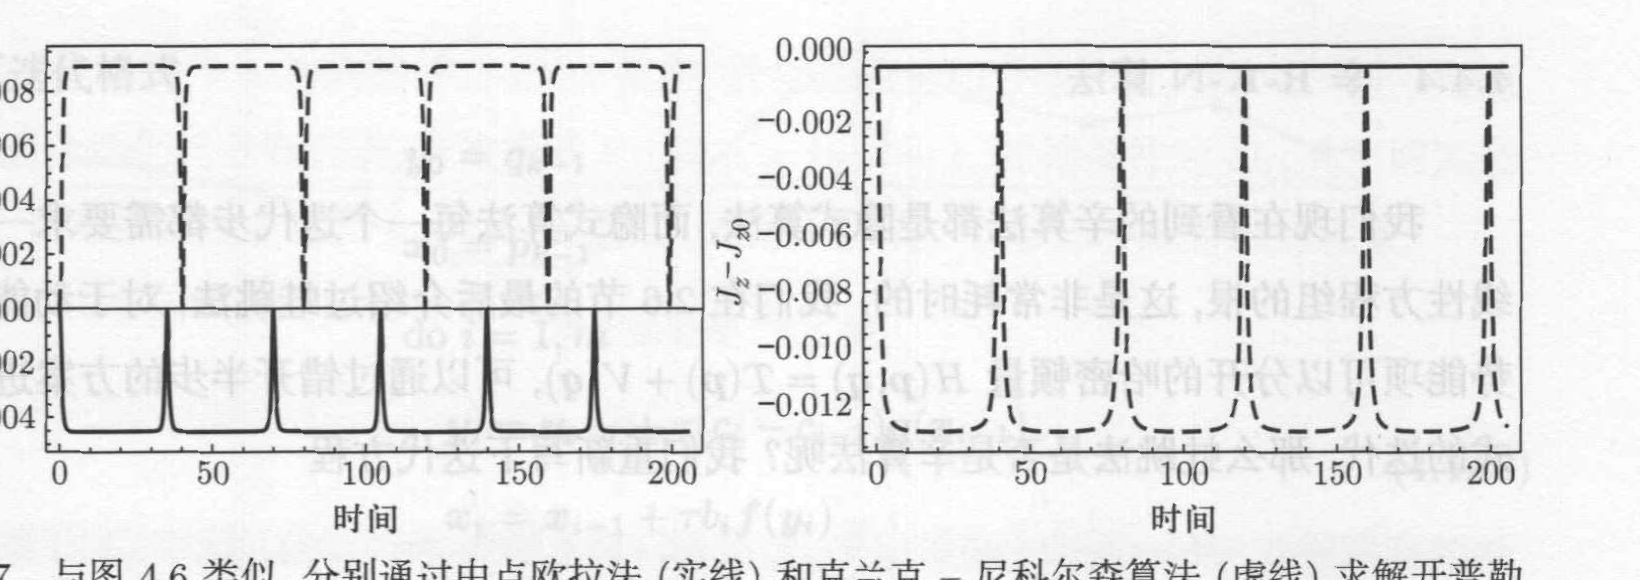
\includegraphics[width=0.88\linewidth]{figures/fig4_7_cn.png}
\caption{与图 4.6 类似，分别通过中点 Euler 法（实线）和 Crank--Nicolson 算法（虚线）求解 Kepler 问题，时间步长固定为 0.2}
\label{fig:cn-kepler}
\end{figure}

\subsection{辛 R--K 算法}

我们现在来考察一般形式的 R--K 算法在满足什么条件时会是辛算法。重新写下 R--K 算法的迭代公式
\begin{equation}
\begin{cases}
\displaystyle g_i=y_{n-1}+\tau\sum_{j=1}^{m}a_{ij}f(g_j),\\[6pt]
\displaystyle y_n=y_{n-1}+\tau\sum_{i=1}^{m}b_i f(g_i).
\end{cases}
\tag{4.4.20}
\end{equation}
取微分
\begin{equation}
\begin{cases}
\displaystyle \mathrm dg_i=\mathrm dy_{n-1}+\tau\sum_{j=1}^{m}a_{ij}\,\mathrm df_j,\\[6pt]
\displaystyle \mathrm dy_n=\mathrm dy_{n-1}+\tau\sum_{i=1}^{m}b_i\,\mathrm df_i,
\end{cases}
\tag{4.4.21}
\end{equation}
然后计算外积
\begin{align}
\mathrm dy_n^{\mathrm T}J\,\mathrm dy_n
&=\mathrm dy_{n-1}^{\mathrm T}J\,\mathrm dy_{n-1}
 +\tau\sum_i b_i\bigl(\mathrm dy_{n-1}^{\mathrm T}J\,\mathrm df_i+\mathrm df_i^{\mathrm T}J\,\mathrm dy_{n-1}\bigr)
 +\tau^2\sum_{i,j}b_ib_j\mathrm df_i^{\mathrm T}J\,\mathrm df_j\notag\\
&=\mathrm dy_{n-1}^{\mathrm T}J\,\mathrm dy_{n-1}
 +\tau\sum_i b_i\bigl(\mathrm dg_i^{\mathrm T}J\,\mathrm df_i+\mathrm df_i^{\mathrm T}J\,\mathrm dg_i\bigr)\notag\\
&\quad+\tau^2\sum_{i,j}(b_ib_j-b_i a_{ij}-b_j a_{ji})\mathrm df_i^{\mathrm T}J\,\mathrm df_j.
\tag{4.4.22}
\end{align}
上式第三项中的系数正好是我们在稳定性分析中见过的 $M$ 矩阵，而第二项括号里的式子由于矩阵 $J$ 的反对称性可知为零。这样外积在 R--K 迭代中守恒便等价于 $M=0$。而基于 Gauß 积分格点的隐式 R--K 算法，如前面所给出的 Radau 5 和 Gauß 6，都满足这个条件，从而是辛算法。

\subsection{辛 R--K--Nyström 算法}

我们现在看到的辛算法都是隐式算法，而隐式算法每一个迭代步都需要求一次非线性方程组的根，这是非常耗时的。我们在 2.6 节的最后介绍过蛙跳法，对于动能项和势能项可以分开的 Hamilton 量 $H(p,q)=T(p)+V(q)$，可以通过错开半步的方案进行显式的迭代。那么蛙跳法是否是辛算法呢？我们重新写下迭代方程
\begin{equation}
\begin{cases}
 p_n=p_{n-1}-\tau\nabla V(q_{n-1/2}),\\
 q_{n+1/2}=q_{n-1/2}+\tau\nabla T(p_n).
\end{cases}
\tag{4.4.23}
\end{equation}
等式两端取微分，有
\begin{equation}
\begin{cases}
 \mathrm dp_n=\mathrm dp_{n-1}-\tau\nabla\nabla V\,\mathrm dq_{n-1/2},\\
 \mathrm dq_{n+1/2}=\mathrm dq_{n-1/2}+\tau\nabla\nabla T\,\mathrm dp_n.
\end{cases}
\tag{4.4.24}
\end{equation}
定义 $y_n=(p_n\;q_{n+1/2})^{\mathrm T}$，那么上式等价于
\begin{equation}
S=\frac{\partial y_n}{\partial y_{n-1}}
=\begin{pmatrix}I&0\\ \tau\nabla\nabla T&I\end{pmatrix}
 \begin{pmatrix}I&-\tau\nabla\nabla V\\0&I\end{pmatrix}.
\tag{4.4.25}
\end{equation}
借助 $V,T$ 两函数 Hessian 矩阵的对称性，容易检验 $S$ 是一个辛矩阵，从而蛙跳法可以看作一个辛算法。注意，由于 $y$ 的定义与之前不同，蛙跳法所能确保的守恒量也会相应变化。例如，对于谐振子，
\begin{equation}
H(q,p)=\frac{p^2}{2}+\frac{q^2}{2},
\tag{4.4.26}
\end{equation}
蛙跳法给出如下的修正 Hamilton 量守恒：
\begin{equation}
\widetilde H=\frac12\bigl[p_n^2+q_{n+1/2}^2-\tau p_nq_{n+1/2}\bigr].
\tag{4.4.27}
\end{equation}

那么这种思路是否可以推广到高阶？答案是肯定的，这就是所谓显式 Runge--Kutta--Nyström 算法。记 $g(p)=\nabla T(p),f(q)=-\nabla V(q)$，有如下迭代格式：
\begin{equation}
\begin{aligned}
y_0&=q_{k-1},\\
x_0&=p_{k-1},\\
\text{do }i&=1,m,\\
y_i&=y_{i-1}+\tau(c_i-c_{i-1})g(x_{i-1}),\\
x_i&=x_{i-1}+\tau b_i f(y_i),\\
\text{end},\\
q_k&=y_m+\tau(1-c_m)g(x_m),\\
p_k&=x_m.
\end{aligned}
\tag{4.4.28}
\end{equation}
此处 $c_i,b_i$ 的含义与通常 R--K 算法中的类似，并默认取 $c_0=0$。令 $m=1,b_1=1,c_1=1/2$ 便给出了蛙跳法。实践上也常用 $m=3$ 的格式，对应于
\[
c=\begin{pmatrix}\frac12+\gamma\\[2pt]\frac12\\[2pt]\frac12-\gamma\end{pmatrix},\qquad
b=\begin{pmatrix}1+2\gamma\\-1-4\gamma\\1+2\gamma\end{pmatrix},
\]
式中 $\gamma$ 为三次方程 $48\gamma^3-24\gamma^2+1=0$ 的实根，
\[
\gamma=\frac{2^{1/3}+2^{-1/3}-1}{6}\approx0.175604.
\]
这个格式具有四阶精度。\footnote{对于此类算法感兴趣的读者可以参考 Okunbor D. and Skeel R. D. Explicit canonical methods for Hamiltonian systems. \textit{Math. Comp.}, 1992, 59: 439.}

\begin{exerciseBox}[练习 4.3]
试编程实现上述算法，并依旧以 Kepler 问题检验其精度。
\end{exerciseBox}

\section*{大作业：FPU 模型}
\addcontentsline{toc}{section}{大作业：FPU 模型}

这一题中我们讨论在计算机上实现的第一个计算物理问题：FPU（Fermi--Pasta--Ulam）模型。\footnote{但在计算机上模拟实现的是另一位女士 Mary Tsingou。关于这段历史可参见 Dauxois T. Fermi, Pasta, Ulam, and a mysterious lady. \textit{Physics Today}, 2008, 61: 55.}这个模型讨论的是一个弹簧振子链，如图 4.8 所示。

 $n$ 个单位质量的质点通过相同的弹簧相互连接，首末两端固定。记 $j$ 号质点偏离平衡位置的距离为 $q_j$，并定义 $q_0=q_{n+1}=0$。系统的 Hamilton 量写成
\begin{equation}
H_\alpha=\frac12\sum_{j=1}^{n}p_j^2+\frac12\sum_{j=0}^{n}(q_j-q_{j+1})^2+\frac\alpha3\sum_{j=0}^{n}(q_j-q_{j+1})^3,
\tag{1}
\end{equation}
或者
\begin{equation}
H_\beta=\frac12\sum_{j=1}^{n}p_j^2+\frac12\sum_{j=0}^{n}(q_j-q_{j+1})^2+\frac\beta4\sum_{j=0}^{n}(q_j-q_{j+1})^4,
\tag{2}
\end{equation}
分别称为 $\alpha$--FPU 模型或 $\beta$--FPU 模型。

\begin{figure}[htbp]
\centering
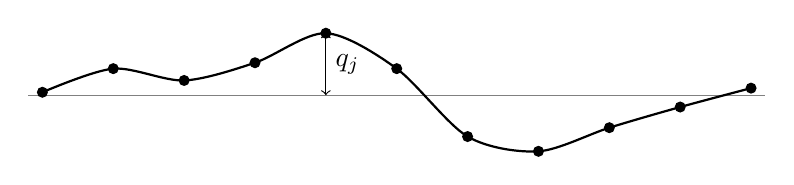
\begin{tikzpicture}[x=0.9cm,y=0.75cm]
\draw[gray] (-0.2,0)--(10.2,0);
\foreach \x/\y in {0/0.05,1/0.45,2/0.25,3/0.55,4/1.05,5/0.45,6/-0.7,7/-0.95,8/-0.55,9/-0.2,10/0.12}{
  \fill (\x,\y) circle (2pt);
}
\draw[thick] plot[smooth] coordinates {(0,0.05)(1,0.45)(2,0.25)(3,0.55)(4,1.05)(5,0.45)(6,-0.7)(7,-0.95)(8,-0.55)(9,-0.2)(10,0.12)};
\draw[<->] (4,0)--(4,1.05) node[midway,right] {$q_j$};
\end{tikzpicture}
\caption{弹簧振子链}
\label{fig:fpu-chain}
\end{figure}

\begin{enumerate}[label=\arabic*.]
\item 解析或数值证明对于没有高次项（$\alpha$ 或 $\beta$ 为 0）的情形，系统具有守恒量
\begin{equation}
E_k=\frac12\dot Q_k^2+\frac12\omega_k^2Q_k^2,
\tag{3}
\end{equation}
其中有
\begin{equation}
Q_k=\sqrt{\frac{2}{n+1}}\sum_{j=1}^{n}q_j\sin\frac{\pi k j}{n+1},\qquad
\omega_k=2\sin\frac{\pi k}{2(n+1)}.
\tag{4}
\end{equation}
\jiaokan{原印本在式 (4) 中将正弦模展开的归一化系数印为 $\sqrt{2/n}$。由固定端点 $q_0=q_{n+1}=0$ 下离散正弦基的正交关系 $\sum_{j=1}^{n}\sin(\pi kj/(n+1))\sin(\pi \ell j/(n+1))=(n+1)\delta_{k\ell}/2$，此处应为 $\sqrt{2/(n+1)}$。}
我们通常将不同的 $k$ 称为不同的声子模式。

\item Fermi 相信，引入非谐项后，系统的能量可以从一个声子模式扩散到全体声子模式上去，从而实现对热平衡过程的模拟。在 FPU 最初的报告中，他们选取 $\alpha$--FPU 模型，令 $\alpha=0.25,n=32,Q_1(0)=4$，而其他 $Q_k(0)$ 以及全部 $\dot Q_k(0)$ 都为零，计算了 $t\in[0,160\times2\pi/\omega_1]$ 的时间内系统的运动。\footnote{这个计算耗费了当时（1953 年）最强大的计算机 MANIAC I 整天的时间。}试重复这个计算，在同一张图上画出 $E_1,E_2,E_3,E_4$ 随时间的变化，时间轴的单位取为 $2\pi/\omega_1$。说明这段时间内有一个时刻几乎全部能量都回到了 $k=1$ 的模式上，并给出具体时刻和能量比例。

\item 给出你认为对这个结果的所有可能解释。（本问不以正误计分，在完成这一问之前请不要往下做。）

\item 1961 年，Tuck 等人将计算的时间长度进一步向前推进。采用前述参数，给出 $t\in[0,4000\times2\pi/\omega_1]$ 的时间中 $E_1$ 的变化图像。说明这段时间内存在一个更大的回归周期，给出具体的回归时刻和能量比例。

\item 非线性系统的动力学行为往往强烈依赖于参数和初始条件的选取。取 $Q_1=20$，其他参数不变。试算并从模式能量的角度描述系统的演化。在多长的时间后系统表现出混沌的特性？讨论此时 $\langle E_k\rangle$ 与 $k$ 的关系，是否和能均分定理相符？

\item 我们将目光转向 $\beta$--FPU 模型。自行选择参数，验证 $\beta$--FPU 模型中也有与之前类似的现象。

\item 论证对于 $n$ 为偶数的 $\beta$--FPU 模型，若初始能量均分布在偶/奇次模式上，则随时间演化后仍然分布在偶/奇次模式上。取 $n=16,\beta=1$，初始条件为 $Q_{11}=1$ 而其余为零，在对数标度上画出 9 至 13 次模式上能量的演化，解释你所观察到的现象。

\item $\beta$--FPU 模型可以看作著名的 KdV 方程
\begin{equation}
\partial_tu+u\partial_xu+\delta^2\partial_{xxx}u=0
\tag{5}
\end{equation}
的离散形式。从而，在恰当的参数下我们能在 $\beta$--FPU 模型中看到 KdV 方程特有的孤子解。取 $n=128$，分别对 $\beta=0,1$，考虑如下形式的初始条件：
\begin{align}
q_i&=B\cos\frac{\pi k(i-n/2)}{n+1}\Big/\cosh\left[\sqrt{\frac32B\omega_k(i-n/2)}\right],\notag\\
p_i&=-\frac{B}{\cosh\left[\sqrt{\frac32B\omega_k(i-n/2)}\right]}
\Biggl\{\omega_k\left(1+\frac3{16}\omega_k^2B^2\right)\sin\frac{\pi k(i-n/2)}{n+1}\notag\\
&\qquad\qquad\qquad\quad+\sqrt{\frac32}B\cos\frac{\pi k(i-n/2)}{n+1}\sin\frac{\pi k}{n+1}
\tanh\left[\sqrt{\frac32B\omega_k(i-n/2)}\right]\Biggr\}.
\tag{6}
\end{align}
其中取 $B=0.5,k=11$，计算系统的运动。用合适的图表展示波包的运动、反射、扩散等过程并讨论之。
\end{enumerate}

% R13 extends through source PDF scan p.180 / printed p.165, completing Chapter 4.
